%%% The main file. It contains definitions of basic parameters and includes all other parts.

%% Settings for single-side (simplex) printing
% Margins: left 40mm, right 25mm, top and bottom 25mm
% (but beware, LaTeX adds 1in implicitly)
\documentclass[12pt,a4paper]{report}
\setlength\textwidth{145mm}
\setlength\textheight{247mm}
\setlength\oddsidemargin{15mm}
\setlength\evensidemargin{15mm}
\setlength\topmargin{0mm}
\setlength\headsep{0mm}
\setlength\headheight{0mm}
% \openright makes the following text appear on a right-hand page
\let\openright=\clearpage

%% Settings for two-sided (duplex) printing
% \documentclass[12pt,a4paper,twoside,openright]{report}
% \setlength\textwidth{145mm}
% \setlength\textheight{247mm}
% \setlength\oddsidemargin{14.2mm}
% \setlength\evensidemargin{0mm}
% \setlength\topmargin{0mm}
% \setlength\headsep{0mm}
% \setlength\headheight{0mm}
% \let\openright=\cleardoublepage

%% Character encoding: usually latin2, cp1250 or utf8:
\usepackage[utf8]{inputenc}

%% Further useful packages (included in most LaTeX distributions)
\usepackage{amsmath}        % extensions for typesetting of math
\usepackage{amsfonts}       % math fonts
\usepackage{amsthm}         % theorems, definitions, etc.
\usepackage{bbding}         % various symbols (squares, asterisks, scissors, ...)
\usepackage{bm}             % boldface symbols (\bm)
\usepackage{graphicx}       % embedding of pictures
\graphicspath{{../img/}}
\usepackage{fancyvrb}       % improved verbatim environment
\usepackage[backend=bibtex, sorting=nyt, style=reading, citestyle=authoryear-comp, entrykey=false, maxbibnames=99, maxcitenames=3]{biblatex} % citation style AUTHOR YEAR
\bibliography{bibliography.bib}
\usepackage[nottoc]{tocbibind} % makes sure that bibliography and the lists
			    % of figures/tables are included in the table
			    % of contents
\usepackage{dcolumn}        % improved alignment of table columns
\usepackage{booktabs}       % improved horizontal lines in tables
\usepackage{paralist}       % improved enumerate and itemize
\usepackage[usenames]{xcolor}  % typesetting in color
\usepackage{tocloft}        % for \cftchapnumwidth
\usepackage{amssymb}        % for \varnothing
\usepackage{hyphenat}       % for \hyp
\usepackage{float}          % for {figure}[H]
\usepackage{enumerate}      % for {enumerate}[(a)]
\usepackage[framemethod=default]{mdframed} % for {mymdframed}
\usepackage{framed}         % for {framed}
\usepackage[justification=justified]{caption} % for justified captions
\usepackage{skak}           % for typesetting Chess
\usepackage{adjustbox}      % for text-sized Chess symbols
\usepackage{epigraph}       % for \epigraph
\usepackage[acronym, toc]{glossaries}
% see https://www.sharelatex.com/learn/Glossaries
\makeglossaries

\newacronym{lp}{LP}{linear program}
\newacronym{nlhe}{NLHE}{No-Limit Texas Hold'em}
\newacronym{lhe}{LHE}{Limit Texas Hold'em}
\newacronym{efg}{EFG}{extensive-form game}
\newacronym{cfr-d}{CFR-D}{counterfactual regret decomposition}
\newacronym{ne}{NE}{Nash equilibrium}
\newacronym{cbv}{CBV}{counterfactual best-response value}
\newacronym{cfr}{CFR}{counterfactual regret minimization}
\newacronym{sm}{SM}{subgame margin}
\newacronym{dtm}{DTM}{depth to~mate}
\newacronym{br}{BR}{best response}
\newacronym{mccfr}{MCCFR}{Monte Carlo counterfactual regret minimization}
\newacronym{nfg}{NFG}{normal-form game}
\newacronym{rps}{RPS}{Rock-Paper-Scissors}
\newacronym{ai}{AI}{artificial intelligence}
\newacronym{cgt}{CGT}{combinatorial game theory}
\newacronym{cnn}{CNN}{convolutional neural network}
\newacronym{isp}{ISP}{Internet Service Provider}
\newacronym{vlp}{VLP}{vector linear program}

\usepackage{mathtools}

\hyphenation{
  e-qui-li-brium
  im-per-fect
  in-for-ma-tion
  end-game
  end-games
  da-ta-ba-se
  back-pro-pa-ga-te
  back-pro-pa-ga-ted
  ex-ten-si-ve
  da-ta-bas-es
}

%%% Basic information on the thesis

% Thesis title in English (exactly as in the formal assignment)
\def\ThesisTitle{Solving Endgames in Large \\Imperfect-Information Games \\such as Poker}

% Author of the thesis
\def\ThesisAuthor{Bc.~Karel Ha}

% Year when the thesis is submitted
\def\YearSubmitted{2016}

% Name of the department or institute, where the work was officially assigned
% (according to the Organizational Structure of MFF UK in English,
% or a full name of a department outside MFF)
\def\Department{Department of Applied Mathematics}

% Is it a department (katedra), or an institute (ústav)?
\def\DeptType{Department}

% Thesis supervisor: name, surname and titles
\def\Supervisor{doc.~Mgr.~Milan Hladík, Ph.D.}

% Supervisor's department (again according to Organizational structure of MFF)
\def\SupervisorsDepartment{Department of Applied Mathematics}

% Study programme and specialization
\def\StudyProgramme{Computer Science}
\def\StudyBranch{Discrete~Models~and~Algorithms}

% An optional dedication: you can thank whomever you wish (your supervisor,
% consultant, a person who lent the software, etc.)
\def\Dedication{%
  \section*{Dedication}
  \epigraphLong{
    The whole thing that makes a~mathematician's life worthwhile is that he gets the grudging admiration of~three or~four colleagues.
  }{Donald Knuth}
  %\begin{itemize}
  %  \item Nyx
  %  \item Milan Hladik
  %  \item parents
  %  \item CERN (hostels, library, facility)
  %\end{itemize}
}

% Abstract (recommended length around 80-200 words; this is not a copy of your thesis assignment!)
\def\Abstract{%
  Endgames have a~distinctive role for players.
  At the late stage of~games, many aspects are finally clearly defined, deeming exhaustive analysis tractable.
  Specialised endgame handling is rewarding for games with perfect information (e.g., Chess databases pre-computed for entire classes of~endings, or dividing Go board into separate independent subgames).

  An~appealing idea would be to extend this approach to imperfect-information games such as the famous Poker:
  play the early parts of~the game, and once the subgame becomes feasible, calculate an~ending solution.
  However, the problem is much more complex for imperfect information.

  \emph{Subgames} need to be generalized to account for \emph{information sets}.
  Unfortunately, such a~generalization cannot be solved straightaway, as it does not generally preserve optimality.
  As a~consequence, we may end up with a~far more exploitable strategy.

  There are currently three techniques to deal with this challenge:
  \begin{enumerate}[(a)]
    \item disregard the problem entirely;
    \item use a~decomposition technique, which sadly retains only the same quality;
    \item or formalize improvements of~strategies into a~so-called \emph{subgame margin}, for which we construct a~``gadget'' game, making it the best possible.
  \end{enumerate}

  The last approach is our own result presented at~the Thirtieth AAAI Conference on~Artificial Intelligence in~2016.
  We experimentally compare the three solutions using a~top participant of~the AAAI-14 Computer Poker Competition, the leading playground for agents in~imperfect-information setting.
}

% 3 to 5 keywords (recommended), each enclosed in curly braces
\def\Keywords{%
  {algorithmic game theory}, {imperfect-information games}, {Nash equilibrium},
  {subgame}, {endgame}, {counterfactual regret minimization}, {Poker}
}

%% The hyperref package for clickable links in PDF and also for storing
%% metadata to PDF (including the table of contents).
\usepackage[pdftex,unicode]{hyperref}   % Must follow all other packages
\hypersetup{breaklinks=true}
\hypersetup{pdftitle={\ThesisTitle}}
\hypersetup{pdfauthor={\ThesisAuthor}}
\hypersetup{pdfkeywords=\Keywords}
\hypersetup{urlcolor=blue}
\hypersetup{hidelinks}

% Definitions of macros (see description inside)
%%% This file contains definitions of various useful macros and environments %%%
%%% Please add more macros here instead of cluttering other files with them. %%%

%%% Minor tweaks of style

% These macros employ a little dirty trick to convince LaTeX to typeset
% chapter headings sanely, without lots of empty space above them.
% Feel free to ignore.
\makeatletter
\def\@makechapterhead#1{
  {\parindent \z@ \raggedright \normalfont
   \Huge\bfseries \thechapter. #1
   \par\nobreak
   \vskip 20\p@
}}
\def\@makeschapterhead#1{
  {\parindent \z@ \raggedright \normalfont
   \Huge\bfseries #1
   \par\nobreak
   \vskip 20\p@
}}
\makeatother

% This macro defines a chapter, which is not numbered, but is included
% in the table of contents.
\def\chapwithtoc#1{
\chapter*{#1}
\addcontentsline{toc}{chapter}{#1}
}

% Draw black "slugs" whenever a line overflows, so that we can spot it easily.
\overfullrule=1mm

%%% Macros for definitions, theorems, claims, examples, ... (requires amsthm package)

\theoremstyle{plain}
\newtheorem{thm}{Theorem}
\newtheorem{lemma}[thm]{Lemma}
\newtheorem{claim}[thm]{Claim}

\theoremstyle{definition}
\newtheorem{defn}{Definition}

\theoremstyle{remark}
\newtheorem*{cor}{Corollary}
\newtheorem*{rem}{Remark}
\newtheorem*{example}{Example}

%%% An environment for proofs

%%% FIXME %%% \newenvironment{proof}{
%%% FIXME %%%   \par\medskip\noindent
%%% FIXME %%%   \textit{Proof}.
%%% FIXME %%% }{
%%% FIXME %%% \newline
%%% FIXME %%% \rightline{$\square$}  % or \SquareCastShadowBottomRight from bbding package
%%% FIXME %%% }

%%% An environment for typesetting of program code and input/output
%%% of programs. (Requires the fancyvrb package -- fancy verbatim.)

\DefineVerbatimEnvironment{code}{Verbatim}{fontsize=\small, frame=single}

%%% The field of all real and natural numbers
\newcommand{\R}{\mathbb{R}}
\newcommand{\N}{\mathbb{N}}

%%% Useful operators for statistics and probability
\DeclareMathOperator{\pr}{\textsf{P}}
\DeclareMathOperator{\E}{\textsf{E}\,}
\DeclareMathOperator{\var}{\textrm{var}}
\DeclareMathOperator{\sd}{\textrm{sd}}

%%% Transposition of a vector/matrix
\newcommand{\T}[1]{#1^\top}

%%% Various math goodies
\newcommand{\goto}{\rightarrow}
\newcommand{\gotop}{\stackrel{P}{\longrightarrow}}
\newcommand{\maon}[1]{o(n^{#1})}
\newcommand{\abs}[1]{\left|{#1}\right|}
\newcommand{\dint}{\int_0^\tau\!\!\int_0^\tau}
\newcommand{\isqr}[1]{\frac{1}{\sqrt{#1}}}

%%% Various table goodies
\newcommand{\pulrad}[1]{\raisebox{1.5ex}[0pt]{#1}}
\newcommand{\mc}[1]{\multicolumn{1}{c}{#1}}

%%%%%%%%%%%%%%%%%%%%%%%%%%%%%%%%%%%%%%%%%%%%%%
% The following section was added by Karel Ha.

% http://tex.stackexchange.com/questions/211414/chapter-0-roman-numerals
\newcommand{\ZeroAlph}[1]{% 0 + \Alph
  \ifcase\value{#1}\relax 0% Chapter 0
  \else\Alph{#1}\fi}% All other chapters
\renewcommand{\thechapter}{\ZeroAlph{chapter}}

% http://tex.stackexchange.com/questions/94464/note-environment-with-mdframed
\global\mdfdefinestyle{exampledefault}{%
  linecolor=lightgray,linewidth=1pt,%
  leftmargin=1cm,rightmargin=1cm,
}
\newenvironment{mymdframed}[1]{%
  \mdfsetup{%
    frametitle={\colorbox{white}{\,#1\,}},
    frametitleaboveskip=-\ht\strutbox,
    frametitlealignment=\raggedright
  }%
  \begin{mdframed}[style=exampledefault]
  }
  {%
  \end{mdframed}
}
\newcommand{\note}[1]{
  \begin{mymdframed}{Note}
    #1
  \end{mymdframed}
}


% mezera v Table of Contents před číslem kapitoly
\renewcommand*\cftchapnumwidth{2.2em}
\renewcommand*\cftsecnumwidth{2.6em}
\def\labelitemi{$\spadesuit$}
\def\labelitemii{$\diamondsuit$}

\newcommand{\HRule}{\rule{\linewidth}{0.5mm}}
\newcommand{\todo}{\textbf{\underline{TODO}}}
\renewcommand{\emptyset}{\varnothing}
\newcommand{\braces}[1]{ \left\{ #1 \right\} }
\newcommand{\I}{\mathcal{I}}
\newcommand{\Mueller}{M\"{u}ller}
\newcommand{\Zurich}{Z\"{u}rich}
\newcommand{\captionWithCite}[2]{ \caption[#1]{#1~(\cite{#2})} }

% black Chess pieces: http://tex.stackexchange.com/questions/150041/how-to-display-black-Chess-pieces-within-normal-text-with-Chessfss?rq=1
\newcommand{\pawnB}[1][1.3ex]{%
  \adjustbox{Trim=4.3pt 2.6pt 4.3pt 0pt,width=#1,margin=0.2ex 0ex 0.2ex 0ex}{\BlackPawnOnWhite}%
}%
\newcommand{\rookB}[1][1.58ex]{%
  \adjustbox{Trim=3.2pt 2.2pt 3.2pt 0pt,width=#1,raise=0ex,margin=0.1ex 0ex 0.1ex 0ex}{\BlackRookOnWhite}%
}%
\newcommand{\knightB}[1][1.85ex]{%
  \adjustbox{Trim=2.3pt 2.35pt 2.5pt 0pt,width=#1,raise=-0.03ex,margin=0.14ex 0ex 0.14ex 0ex}{\BlackKnightOnWhite}%
}%
\newcommand{\bishopB}[1][1.79ex]{%
  \adjustbox{Trim=2.3pt 2pt 2.3pt 0pt,width=#1,raise=-0.12ex,margin=0.1ex 0ex 0.1ex 0ex}{\BlackBishopOnWhite}%
}%
\newcommand{\queenB}[1][2.05ex]{%
  \adjustbox{Trim=1.2pt 2.2pt 1.2pt 0pt,width=#1,raise=-0.08ex,margin=0.1ex 0ex 0.1ex 0ex}{\BlackQueenOnWhite}%
}%
\newcommand{\kingB}[1][1.95ex]{%
  \adjustbox{Trim=2pt 2pt 2pt 0pt,width=#1,raise=-0.06ex,margin=0.13ex 0ex 0.13ex 0ex}{\BlackKingOnWhite}%
}%

\setlength{\epigraphwidth}{0.6\textwidth}
\renewcommand{\textflush}{flushepinormal} % justified text of epigraphs
\let\oldepigraph\epigraph
\renewcommand{\epigraph}[2]{\oldepigraph{#1}{#2}\noindent\ignorespaces}

\def\codeText#1{\texttt{#1}}

\renewcommand\qedsymbol{$\blacksquare$}
\newcommand{\lv}{\left\vert}
\newcommand{\rv}{\right\vert}
\DeclareMathOperator*{\argmin}{arg\,min}
\DeclareMathOperator*{\argmax}{arg\,max}

\hyphenation{
  e-qui-li-brium
  im-per-fect
  in-for-ma-tion
  end-game
  end-games
  da-ta-ba-se
  back-pro-pa-ga-te
  back-pro-pa-ga-ted
  ex-ten-si-ve
}
%%%%%%%%%%%%%%%%%%%%%%%%%%%%%%%%%%%%%%%%%%%%%%


% Title page and various mandatory informational pages
\begin{document}
%%% Title page of the thesis and other mandatory pages

%%% Title page of the thesis

\pagestyle{empty}
\hypersetup{pageanchor=false}
\begin{center}

\centerline{\mbox{
\includegraphics[width=166mm]{../img/logo-en.pdf}}}

\vspace{-8mm}
\vfill

{\bf\Large MASTER THESIS}

\vfill

{\LARGE\ThesisAuthor}

\vspace{15mm}

\HRule \\[0.6cm]
{\LARGE\bfseries\ThesisTitle}
\HRule \\[1.5cm]

\vfill

\Department

\vfill

\begin{tabular}{rl}

Supervisor of the master thesis: & \Supervisor \\
\noalign{\vspace{2mm}}
Study programme: & \StudyProgramme \\
\noalign{\vspace{2mm}}
Study branch: & \StudyBranch \\
\end{tabular}

\vfill

% Zde doplňte rok
Prague \YearSubmitted

\end{center}

\newpage

%%% Here should be a bound sheet included -- a signed copy of the "master
%%% thesis assignment". This assignment is NOT a part of the electronic
%%% version of the thesis. DO NOT SCAN.

%%% A page with a solemn declaration to the master thesis

\openright
\hypersetup{pageanchor=true}
\pagestyle{plain}
\pagenumbering{roman}
\vglue 0pt plus 1fill

\noindent
I declare that I carried out this master thesis independently, and only with the cited
sources, literature and other professional sources.

\medskip\noindent
I understand that my work relates to the rights and obligations under the Act No.~121/2000 Sb.,
the Copyright Act, as amended, in particular the fact that the Charles
University has the right to conclude a license agreement on the use of this
work as a school work pursuant to Section 60 subsection 1 of the Copyright Act.

\vspace{10mm}

\hbox{\hbox to 0.5\hsize{%
In ........ date ............	% FIXME!
\hss}\hbox to 0.5\hsize{%
signature of the author
\hss}}

\vspace{20mm}
\newpage

%%% Mandatory information page of the thesis

\openright

\vbox to 0.5\vsize{
\setlength\parindent{0mm}
\setlength\parskip{5mm}

Title:
{\let\\=\relax \ThesisTitle}

Author:
\ThesisAuthor

\DeptType:
\Department

Supervisor:
\Supervisor, \SupervisorsDepartment

Abstract:
\Abstract

Keywords:
\Keywords

\vss}

\newpage

%%% Dedication

\openright

\noindent
\Dedication

\newpage

\openright
\pagestyle{plain}
\pagenumbering{arabic}
\setcounter{page}{1}


%%% A page with automatically generated table of contents of the master thesis

\tableofcontents

%%% Each chapter is kept in a separate file
\setcounter{chapter}{-1}            % start from chapter 0
\chapter*{Introduction}
\addcontentsline{toc}{chapter}{Introduction}


\chapter{Preliminaries}
\epigraph{
  I can't go to a~restaurant and order food because I keep looking at the fonts on~the menu.
}{Donald Knuth}

\section{General Game Theory}

\subsection{What Is Game Theory?}

The field of Game Theory deals with interactions or conflicts between $2$ or more agents.
\todo

A~\emph{(simultaneous move) game} consists of: \todo
\begin{itemize}
  \item set $P$ of players $\braces{1, 2, \cdots, n}$
  \item actions
  \item payoffs
\end{itemize}

\subsection{Representation of Games}

\todo
Forms:
\begin{itemize}
  \item \acrfull{nfg}
  \item \acrfull{efg}
\end{itemize}

There will be other kinds of representation for extensive form games (see Section~\ref{sec:extensive-form-perf-info} and Section~\ref{sec:extensive-form-imperf-info}).

\section{Examples of~Games}

\todo %Describe the games and how the game-theoretic definitions from above look like in these examples

\begin{itemize}
  \item{Rock-paper-scissors}
  \item{Chess}
  \item{Poker}
\end{itemize}

One of the classic textbook is the extensive \emph{Algorithmic Game Theory} (\cite{AGT07}).
\todo
The following games capture various game-theoretic properties and the ``real-life'' counterparts of these games in the fields such as networking, economy etc.
The examples and figures are taken from \emph{Algorithmic Game Theory} (\cite{AGT07}).

\newcommand{\widthratio}{0.3}
\begin{itemize}
  \item \emph{Prisoner's dilemma} \todo
    \begin{figure}[H]
      \centering
      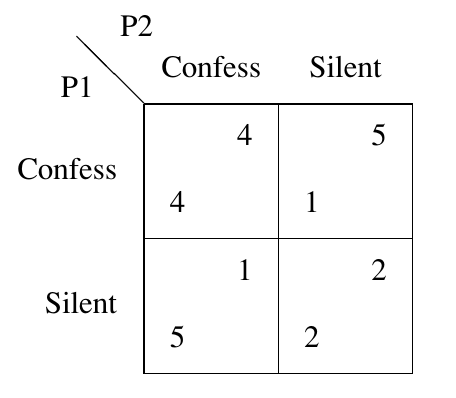
\includegraphics[width=\widthratio\paperwidth]{../img/prisoner.png}
      \caption{Prisoner's dilemma}
      \label{fig:prisoner}
    \end{figure}

    \begin{figure}[H]
      \centering
      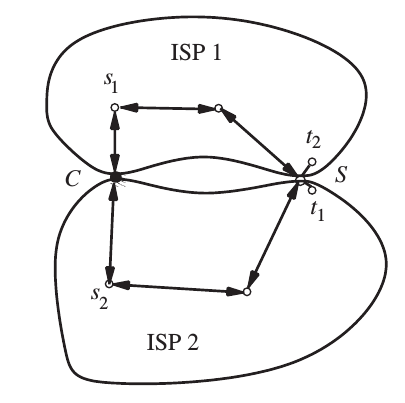
\includegraphics[width=\widthratio\paperwidth]{../img/isp.png}
      \caption{ISP routing game}
      \label{fig:isp-routing}
    \end{figure}


  \item \emph{Pollution game} is a multi-player version of Prisoner's dilemma \todo

  \item An~example of a~coordination game is the \emph{Battle of sexes}.

    \begin{figure}[H]
      \centering
      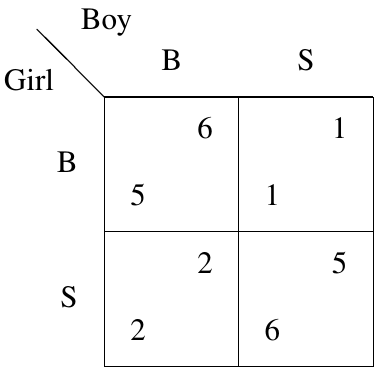
\includegraphics[width=\widthratio\paperwidth]{../img/battle-of-sexes.png}
      \caption{Battle of sexes}
      \label{fig:battle-of-sexes}
    \end{figure}

  \item Another coordination game is the \emph{Routing congestion game}, taken from the world of networking

    \begin{figure}[H]
      \centering
      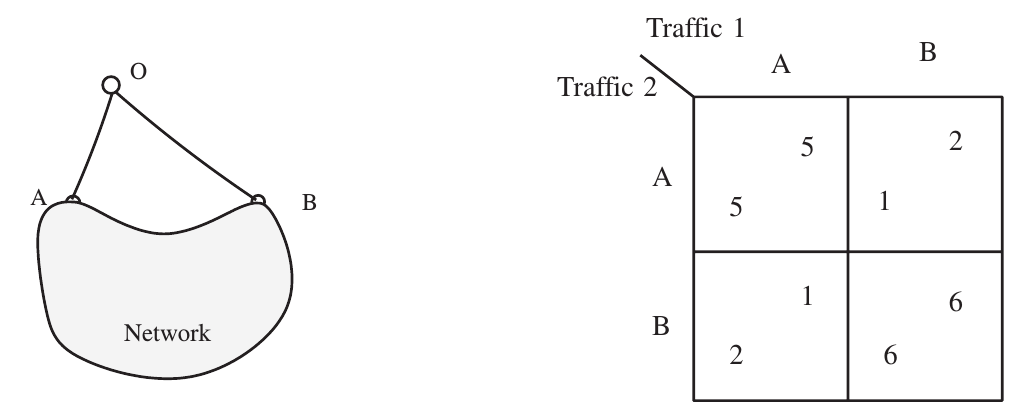
\includegraphics[width=0.65\paperwidth]{../img/routing-congestion-game.png}
      \caption{Routing congestion game}
      \label{fig:routing-congestion}
    \end{figure}

  \item \emph{Matching pennies} can be considered as a $2$-choice reduction of Rock-paper-scissors.

    \begin{figure}[H]
      \centering
      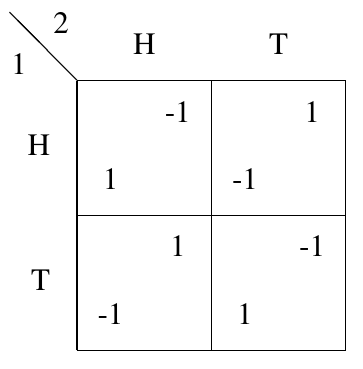
\includegraphics[width=\widthratio\paperwidth]{../img/matching-pennies.png}
      \caption{Matching pennies}
      \label{fig:matching-pennies}
    \end{figure}

  \item \emph{Pricing game} is an~example of a~game without a~(mixed) \acrshort{ne}.

    \begin{figure}[H]
      \centering
      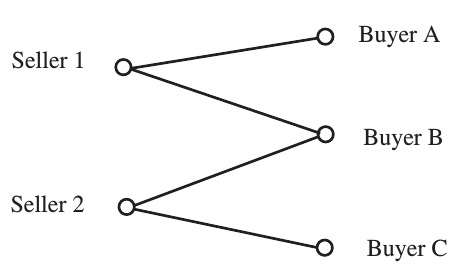
\includegraphics[width=\widthratio\paperwidth]{../img/pricing-game.png}
      \caption{Pricing game}
      \label{fig:pricing-game}
    \end{figure}

  \item \emph{Traffic light}

    \begin{figure}[H]
      \centering
      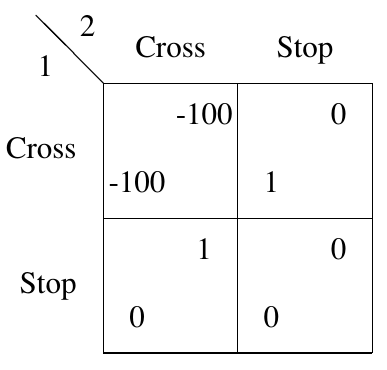
\includegraphics[width=\widthratio\paperwidth]{../img/traffic-light.png}
      \caption{Traffic light}
      \label{fig:traffic-light}
    \end{figure}

  \item \emph{Ultimatum game}
\end{itemize}
\section{The Game of Go}
\label{sec:Go}

\subsection{Rules}

\emph{Black} and \emph{White} place pieces (\emph{stones}) on the unoccupied intersections (\emph{points}) of a~\emph{board} with a~$19\times19$ grid of~lines.
Players take turns, Black moves first.
There are only 2 basic rules of Go:
\begin{description}
  \item [The rule of liberty]
    Every stone remaining on the board must have at least one open point (an~intersection, called a~\emph{liberty}) directly next to it (up, down, left, or right), or must be part of a~connected group that has at least one such liberty next to it.
    \begin{figure}[H]
      \centering
      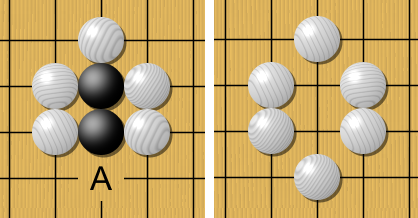
\includegraphics[width=.5\textwidth]{../img/Go_rule_of_liberty.png}
      \caption{The rule of liberty}
      \label{fig:Go-rule-liberty}
    \end{figure}

    Stones or groups of stones which lose their last liberty are removed from the board.

  \item [The ``ko'' rule]
    The stones on the board must never repeat a~previous position of~stones.
    This is to prevent unending cycles.
    \begin{figure}[H]
      \centering
      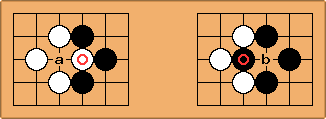
\includegraphics[width=.5\textwidth]{../img/Go_ko_rule.png}
      \caption{The ``ko'' rule}
      \label{fig:Go-Ko-rule}
    \end{figure}

\end{description}

\subsection{Scoring, Ranks and Handicaps}

There are several \textbf{scoring rules} to determine the winner of a~game.
In the match of~AlphaGo against Lee Sedol,%
\footnote{See Chapter~\ref{ch:AlphaGo}.}
the \emph{area scoring} was used.
Under area scoring system, player's score is:
\begin{itemize}
  \item the number of stones that the player has on the board
  \item plus the number of~empty intersections surrounded by that player's stones
  \item plus \emph{komi(dashi)} points%
    \footnote{a~compensation for the first move advantage of~the Black player}
    for the White player
\end{itemize}

\emph{Elo rating} can be used to denote players' \textbf{ranks}.
Alternatively, \emph{kyu/dan} (in~Japanese) or \emph{gup/dan} (in~Korean) system is also vastly popular:
\begin{figure}[H]
  \centering
  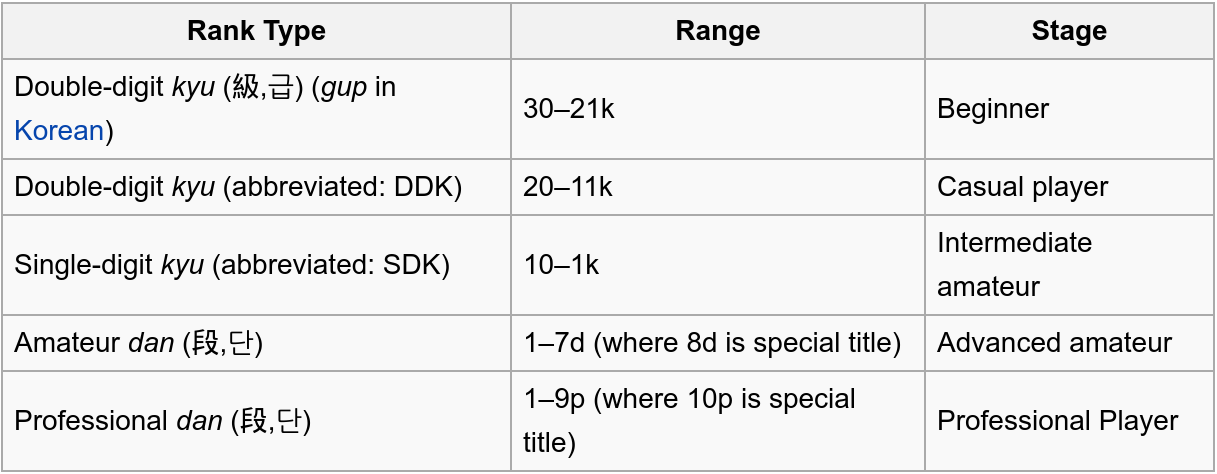
\includegraphics[width=.8\textwidth]{../img/Go_kyu_dan.png}
  \caption{Kyu/Gup and Dan ranks}
  \label{fig:Go-ranks}
\end{figure}

\textbf{Handicap} system is used to even up differences in ranks:
Black can place 1 or more stones in advance as a~compensation for White's greater strength.

\section{Combinatorial Game Theory}
\label{sec:CGT}
\todo



%%% Part I %%%
\part{Perfect Endgames of~Perfect-Information Games}
\chapter{Setting the Scene for Perfect Information}
\epigraphLong{
  In order to improve your game, you must study the endgame before everything else.
  For whereas the endings can be studied and mastered by~themselves, the middle game and opening must be studied in relation to the end game.
}{José Raúl Capablanca}
For many games, solving their late stages (so-called \emph{endgames}) can be done in~a~dynamic online way.
In other words, we are often able to postpone the computation of~the endgame strategy until the endgame itself is reached in~the play.

On the other hand, endgames can be also pre-computed (often up to a~perfect play) and cached for later.
Such a~``memoization'' approach is notably fruitful in~popular games such as Chess.

\section{Extensive Form for Perfect-Information}
\label{sec:extensive-form-perf-info}
\epigraph{Trees that are slow to grow bear the best fruit.}
{Molière}
Games with perfect information can be naturally represented with a~\emph{game tree}:
\begin{figure}[H]
  \centering
  \scriptsize
  \def\svgwidth{.9\textwidth}
  \input{../img/game_tree_nim_5.pdf_tex}
  \def\captionTitle{Game tree of~(1,2)-Nim with 1~heap of 5~stones}
  \caption[\captionTitle]{\captionTitle{} (rendered by \codeText{Gambit} using the included example \codeText{nim.efg})}
  \label{fig:game-tree-nim-5}
\end{figure}
\noindent
The representation with a~(directed) tree (rather than with a~pay-off matrix) is called an extensive form.

Formally, an~\emph{extensive-form game} (\cite[p.~200]{Osborne1994course}) for a~perfect-information game consists of:
\begin{itemize}
  \item a~finite set of~\emph{players}~$P$,

  \item a~finite set $H$ of~all possible \emph{histories} (i.e. paths from the root to vertices of~the game tree), where
    \begin{itemize}
      \item each history consists of~individual \emph{actions} (i.e. tree edges),
      \item $\emptyset \in H$ (the root of~the game tree),
      \item relation~$h \sqsubseteq h'$ denotes that history~$h$ is a~prefix of $h'$,
      \item if $h' \in H$ and $h \sqsubseteq h'$, then $h \in H$,
      \item set $Z \subseteq H$ is the set of \emph{terminal histories}, i.e. histories that are not prefixes of~any other histories.
    \end{itemize}

  \item the set of available actions $A(h) = \braces{a: (h, a) \in H}$ for every (non-terminal) node $h \in H \setminus Z$ (i.e. edges to~children in the game tree),

  \item a~function $p\colon P \to H \setminus Z$, which assigns an~\emph{acting player} $p(h)$ to each non-terminal history~$h$.

  \item a~\emph{utility function} $u_i\colon Z \goto \R$.
\end{itemize}
We will also need the notion of~a~strategy, the expected utility and a~best response.
\begin{itemize}
  \item A~(behavior) \emph{strategy}~$\sigma_i$ of player~$i$ defines a~probability distribution over actions $A(h)$ wherever he acts (i.e. at~every node~$h \in H$ with $p(h) = i$).
    The set~$\Sigma_i$ contains all possible strategies for player~$i$.

  Additionally, a~strategy can be \emph{pure} (just one action is strictly chosen everywhere) or \emph{mixed} (a~probability distribution over pure strategies).

  \item A~\emph{strategy profile} $\sigma$ is a~vector of~players' strategies:
    $\sigma = (\sigma_1, \sigma_2, \ldots, \sigma_ {\abs{P}})$.
    The set of~all such possible strategy profiles is denoted by~$\Sigma$.
    Hence, it is the Cartesian product $\Sigma = \prod_{i \in P} \Sigma_i$.

    By~$\sigma_{-i}$ we denote the strategy profile of~$i$'s opponents:
    \[ \sigma_{-i} = (\sigma_1, \sigma_2, \ldots \sigma_{i-1}, \sigma_{i+1}, \ldots \sigma_ {\abs{P}}) \]

  \item We use the symbol $\pi^\sigma$ (resp. $\pi_i^\sigma$) to evaluate the overall (resp. player~$i$'s) probability corresponding to a~strategy profile~$\sigma$.
    The probability $\pi^\sigma(h)$ of~reaching node~$h$ can be decomposed to each player's contribution as
    \[ \pi ^\sigma(h) = \prod _{i \in P} \pi _i ^\sigma (h) \]

    Furthermore, the probability $\pi _{-i} ^\sigma (h)$ (shortly $\pi _{-i} (h)$) is the product of~all players' contribution, except for $i$'s one:
    \[ \pi _{-i} ^\sigma(h) = \prod _{j \ne i} \pi _j ^\sigma (h) \]
    
  \item Given a~strategy profile $\sigma$, the \emph{expected utility}~$u_i (\sigma)$ for player~$i$
    is the sum of~utilities in~the leaves (weighted by the probabilities of~reaching them):
    \[ u_i (\sigma) = \sum _{z \in Z} \pi^\sigma\!(z) \,u_i(z)\]

  \item Player~$i$'s \emph{best response}~$BR _i (\sigma _{-i})$ (briefly $BR _i (\sigma)$) is a~strategy $\sigma _i \in \Sigma _i$ maximizing his expected utility against other players:
    \[ u_i (\sigma) = \max _{\sigma'_i \in \Sigma_i} u_i ((\sigma'_i, \sigma_{-i})) \]
    Provided a~fixed $\sigma_{-i}$, one technique to find some best response is to recursively traverse the game tree and pick each node's most valuable action (with the maximum utility).
\end{itemize}
\note{
  There may be several best responses due to a~multiplicity of~actions with maximum value.
  Let us assume $BR _i (\sigma _{-i})$ denotes any of~them:
  this simplification is not overly harmful, since all best responses lead to the same (maximum) value of~the total utility.
}

Finally, two common properties of~games are:
\begin{itemize}
  \item \emph{two-player} property
  \item \emph{zero-sum} property:
    For any profile $\sigma \in \Sigma$, players' utilities cancel out
    \[ \sum _{i \in P} u _i (\sigma) = 0 \]
\end{itemize}
In particular, two-player zero-sum games capture the~antagonistic behavior:
what one player gains, the other one loses.
Typical examples are rock-paper-scissors, matching pennies, Chess, Go, heads-up poker etc.

\section{Subgames}
\epigraphLong{
  At that time I did not suspect that it [``An Oligopoly Model with Demand Inertia'' (\cite{Selten1968oligopoly})] often would be quoted, almost exclusively for the definition of subgame perfectness.
}{Reinhard Justus Reginald Selten}
In~the perfect-information setting, a~\emph{subgame} is a~game corresponding to a~subtree of~the game tree.
Specifically, any node in~the tree induces its own subgame:
\begin{figure}[H]
  \centering
  \scriptsize
  \def\svgwidth{.7\textwidth}
  \input{../img/extended-form_subgame.pdf_tex}
  \def\captionTitle{Subgame induced by node~$2_2$}
  \caption[\captionTitle]{\captionTitle{}\\ (\href{https://en.wikipedia.org/wiki/Subgame_perfect_equilibrium}{https://en.wikipedia.org/wiki/Subgame\_perfect\_equilibrium})}
  \label{fig:ext-form-subgame}
\end{figure}

\note{
  For the upcoming proofs, we define the notation for \emph{the~restriction of the expected utility} on a~subgame rooted in node~$h\in H$:
  \[ u_i^h(\sigma) = \sum _{z \in Z,\; h \sqsubseteq z} \pi^\sigma\!(h,z) \,u_i(z) \]
  where $\pi^\sigma(h,z)$ is the probability of~reaching $z$ from node~$h$ under $\sigma$.
}

If we fix opponents' strategies, it is only beneficial to re-solve subgames:%
\footnote{This property also holds for imperfect-information subgames.}
\begin{thm}[subgame re-solving and utility]
  \label{thm:perf-info-subgames-utility}
  The re-computed sub-strategies can be ``placed back'' into the full-game strategy, without decreasing the total expected utility.
\end{thm}
\begin{proof}
  Let $\sigma$ be any~full-game strategy and $\sigma_S$ be its restriction to a~subgame~$S$ rooted at node~$r$.
  Assume we found a~better (or even optimal) strategy $\sigma^*$ for the subgame~$S$.
  In other words, the arising expected utility of~any player~$i$ is better within $S$:
  \begin{equation}
    \label{eq:opt-val-of-subgame}
    u_i^r(\sigma^*) \ge u_i^r(\sigma_S)
  \end{equation}
  The new re-combined strategy $\sigma'$ (i.e. $\sigma^*$ within~$S$, and the original $\sigma$ elsewhere) cannot decrease $i$'s utility:
  \begin{align*}
    u_i(\sigma')
    %
    &= \sum _{z \in Z} \pi^{\sigma'}\!(z) \,u_i(z)
    %
    = \sum _{z \in Z \cap S} \pi^{\sigma'}\!(z) \,u_i(z)
    + \sum _{z \in Z \setminus S} \pi^{\sigma'}\!(z) \,u_i(z) \\
    %
    &= \left[ \pi^{\sigma'}\!(r)\sum _{z \in Z \cap S} \pi^{\sigma^*}\!(r, z) \,u_i(z) \right]
    + \sum _{z \in Z \setminus S} \pi^{\sigma'}\!(z) \,u_i(z) \\
    %
    &= \pi^{\sigma}\!(r) \,u_i^r(\sigma^*)
    + \sum _{z \in Z \setminus S} \pi^{\sigma}\!(z) \,u_i(z)
    %
    \stackrel{\mathclap{\mathrm{(\ref{eq:opt-val-of-subgame})}}} {\ge}
    \pi^{\sigma}\!(r) \,u_i^r(\sigma_S)
    + \sum _{z \in Z \setminus S} \pi^{\sigma}\!(z) \,u_i(z) \\
    %
    &= \sum _{z \in Z \cap S} \pi^{\sigma}\!(z) \,u_i(z)
    + \sum _{z \in Z \setminus S} \pi^{\sigma}\!(z) \,u_i(z)
    %
    = u_i(\sigma)
  \end{align*}
  Therefore, combining the new $\sigma^*$ with the full-game $\sigma$ does not decrease the total expected utility.
\end{proof}

The perfect-information setting offers one additional advantage over the imperfect information:
no opponent can exploit the newly computed sub-strategy by adjusting his play (either in~the trunk or in~the subgame).
\begin{thm}[unexploitable subgame re-solving]
  \label{thm:perf-info-subgames-unexploitability}
  Assume we are given a~two-person zero-sum game, its subgame~$S$ rooted at node~$r$ and a~fixed player~$i$.
  Let $\sigma_i$ be the~original strategy, $\sigma_i^*$ the re-computed strategy that only differs within $S$, let $\sigma_{-i} = BR(\sigma _{i})$ and $\sigma_{-i}^* = BR(\sigma^*_{i})$ be opponent's corresponding best responses, and let $\sigma = (\sigma_i, \sigma_{-i})$ and $\sigma^* = (\sigma_i^*, \sigma_{-i}^*)$ be the resulting profiles.

  If $u_i^r (\sigma) \le u_i^r (\sigma^*)$ (player~$i$'s worst-case utility does not decrease in~the subgame), then at~every node $h \in H \setminus S$ we also have $u_i^h (\sigma) \le u_i^h (\sigma^*)$ (player~$i$'s worst-case utilities outside the subgame do not decrease).
\end{thm}
\begin{proof}
  By definition, all best responses produce equal expected utilities, because they all maximize opponent's value.
  We can therefore do calculations of~utilities with respect to any~arbitrary best response, e.g. the standard best response retrieved by~the \emph{backward induction}\footnotemark.
  \footnotetext{This method recursively selects the action with the maximum utility, or any of~them in~the case of~multiplicity.}

  Let $T_h$ be the subtree rooted at~$h$.
  If $T_h$ does not contain $S$ (i.e. $h \not\sqsubseteq r$), then the best responses $\sigma_{-i}$ and $\sigma^*_{-i}$ are identical within $T_h$, which trivially implies $u_i^h (\sigma) = u_i^h (\sigma^*)$.
  On~the other hand, if $T_h$ does contain $S$, we will prove the inequality by~mathematical induction on the height of~$T_h$.

  For the base case, the minimum-height tree containing $S$ is the subgame tree $S \equiv T_r$ itself, where the inequality holds by assumptions.
  For the inductive step, let node~$h$ has $k$ children $h_1, \dots h_k$, and without loss of~generality, $T_{h_1}$ contains $S$.
  By~the induction hypothesis, $u_i^{h_1} (\sigma) \le u_i^{h_1} (\sigma^*)$.
  Because the subtrees of~the remaining children don't contain $S$ (i.e. $h_j \not\sqsubseteq r$ for $j = 2, \dots, k$), $\sigma$ and $\sigma^*$ are equal there.
  Hence, $u_i^{h_j} (\sigma) = u_i^{h_j} (\sigma^*)$ for $j = 2, \dots, k$.
  Therefore, we have
  \begin{equation}
    \label{eq:children-inc-util}
    u_i^{h_j}(\sigma) \le u_i^{h_j}(\sigma^*)
  \end{equation}
  If $i$ is the acting player of~$h$ (i.e. $p(h) = i$), then by~expressing utilities as weighted sums of~children's utilities we get
  \begin{align*}
    u_i^h(\sigma)
    %
    &= \sum _{j = 1, \dots, k} \pi^\sigma\!(h,h_j) \,u_i^{h_j}(\sigma)
    %
    = \sum _{j = 1, \dots, k} \pi^{\sigma^*}\!(h,h_j) \,u_i^{h_j}(\sigma) \\
    %
    &\stackrel{\mathclap{\mathrm{(\ref{eq:children-inc-util})}}} {\le}
    \sum _{j = 1, \dots, k} \pi^{\sigma^*}\!(h,h_j) \,u_i^{h_j}(\sigma^*)
    %
    = u_i^h(\sigma^*)
  \end{align*}
  On the other hand, if the opponent is the one who is acting (i.e. $p(h) \ne i$), he aims to choose the action with $i$'s minimum utility (due to the zero-sum property):
  \begin{align*}
    u_i^h(\sigma)
    %
    = \min _{j = 1, \dots, k} \,u_i^{h_j}(\sigma)
    %
    \stackrel{\mathclap{\mathrm{(\ref{eq:children-inc-util})}}} {\le}
    \min _{j = 1, \dots, k} \,u_i^{h_j}(\sigma^*)
    %
    = u_i^h(\sigma^*)
  \end{align*}
  In either cases $u_i^h(\sigma) \le u_i^h(\sigma^*)$.
\end{proof}

\begin{cor}
  If a~player employs a~re-computed subgame strategy, the opponent has no way to~adjust his strategy, in order to increase his own overall utility.
\end{cor}

This means that we can deal with subgames of~perfect-information games separately, either by~pre-computation or by~dynamic in-play re-solve.
Moreover, we may freely combine the newly found strategies with the original ones:
Theorem~\ref{thm:perf-info-subgames-utility} guarantees they won't be inferior, and Theorem~\ref{thm:perf-info-subgames-unexploitability} guarantees their unexploitability by the opponent.

\note{
  The situation in imperfect-information setting is different:
  in~fact, Claim~\ref{claim:rps-subgame} proves that a~re-solved subgame strategy can be actually exploited.
}

\section{Working Examples}
\epigraph{
  Few things are harder to~put up with than the~annoyance of a~good example.
}{Mark Twain}
Subgame solutions are particularly used in~perfect-information games with an~extensive form such as Chess or Go, where the endgame technique has been used for~long time as one way to~defeat the colossal size of~the game tree.
In these specific domains, endgame solving has~additional significance, as it improves the playing quality of~agents as well.

In Chapter~\ref{ch:Chess}, we will see the power of~subgame pre-computation with the example of~Chess:
solutions to~endings are stored in so-called \emph{endgame tablebase}.
They are used in~real world to~aid professional Chess players, either in~proving their guaranteed victory or in~analysing past games.
Moreover, since tablebases are mathematically proven to be~optimal, they provide a~glimpse into the world of~``perfect Chess'' played by ``all-knowing super-players''.

In contrast, Chapter~\ref{ch:goCGT} demonstrates how the in-play approach to~endgames is beneficial in~the game of~Go.
Once reaching the late stage, the board is partitioned into distinct parts.
The corresponding (and provably independent) subgames are re-solved ``on the fly'', just to be afterwards combined using the \emph{combinatorial game theory}.

Finally, Chapter~\ref{ch:AlphaGo} reviews the modern approach to~computer Go employed by~Google DeepMind:
the Go program \emph{AlphaGo} combines \emph{Monte Carlo tree search} with \emph{neural networks} to~simulate every play position, as if it were an~endgame.
This in particular means that several moves into the future are simulated and the corresponding part of~the game tree is unrolled and expanded.
The rest of~the tree is discarded, effectively leaving only the relevant subgame for the oncoming play.

\chapter{Chess Endgames}

\section{What are Endgames in Chess?}
\epigraph{
  Studying openings is just memorizing moves and looking for traps.
  Studying the endgame is chess.
}{Josh Waitzkin}

The notion of~``endgame'' has no strict definition and greatly differs by various authors.
The common sense says it begins with only few pieces left.
Here are some examples of~various approaches to defining endgames:
\begin{itemize}
  \item
    positions in which each player has less than thirteen points in material (not counting the king)
    (\cite[pp.~7--8]{Speelman1981endgame})
    
  \item
    positions in which the king can be used actively (but there are some famous exceptions to that)
    (\cite[pp.~7--8]{Speelman1981endgame})
    
  \item
    positions having four or fewer pieces other than kings and pawns
    (\cite[p.~5]{Minev2004practical})
    
  \item
    positions without queens
    (\cite{Fine1952middle}),
    
  \item
    positions when each player has less than a queen plus rook in material
    
  \item
    positions when the player who is about to move can force a~win or a~draw against any variation of~moves
    (\cite{Portisch1981six})

  \item 
    positions with these three characteristics~(\cite{Alburt1999just}):

    \begin{enumerate}[(a)]
      \item Endgames favor an~\emph{aggressive} king.
      \item \emph{Passed pawns} increase greatly in importance.
      \item \emph{Zugzwang} is often a factor in endgames and rarely in other stages of the game.
    \end{enumerate}

  \item
    ``Not Quite an Endgame'' (NQE) are positions where each player has at most one piece (other than kings and pawns), and positions with more material where each player has at most two pieces
    (\cite[pp.~7--8]{Flear2007practical})
\end{itemize}

Nevertheless, endgames have one thing in~common:
the complexity~of the board is often manageable by~computers, making it feasible to compute the perfect strategy.

\section{Endgame Tablebases}
{
  \setlength{\epigraphwidth}{0.5\textwidth}
  \epigraph{
    Studying the endgame is like cheating.
  }{Michael J.~Frannett}
}

An~\emph{endgame tablebase} is a~database of~pre-calculated, exhaustively analysed chess endgames stored as tables of~positions together with the best consequent moves.
Upon reaching an~arbitrary tablebase position, the~database thus provides an~optimal strategy to play perfect chess.

Tablebases are designed for a~given set of~pieces, e.g. \king King and \queen Queen versus \kingB King (KQ-K).
There are 3 basic steps in their process of~creation:
\begin{enumerate}[1]
  \item \textbf{Generation}:
    Computer generates all legal positions for the given pieces.
    For each position, the tablebase evaluates the situation separately for White-to-move and Black-to-move.

    In~the case of~KQ-K, the number of~positions amounts to $\approx 40000$.
    Such number is due to the symmetry argument~(\cite{Levy2009computers}):
    assume the \kingB{} is on~square a1, b1, c1, d1, b2, c2, d2, c3, d3, or d4 (see diagram on~Figure~\ref{fig:non-symmetric-black-king}).
    Other squares are equivalent by symmetry of~rotation or reflection.

    Now there are $\approx 60$ remaining squares for the \king{} and at most $62$ squares for the \queen.
    Therefore, there are at most $10 \times 60 \times 62 = 37200$ KQ-K positions.
    \begin{figure}[H]
      \centering
      \newgame
      \fenboard{8/8/8/8/3k4/2kk4/1kkk4/kkkk4 - - - 0 0}
      \showboard
      \captionWithCite{Non-symmetric positions for \kingB}{Levy2009computers}
      \label{fig:non-symmetric-black-king}
    \end{figure}

    Adding one new piece into a~\emph{pawnless} endgame multiplies the count of~positions by $\approx 60$ (the approximate quantity of~unoccupied positions).
    Pawns would break the front-back and diagonal symmetries, because they care about direction in their moves~(\cite{Muller2006EGTB}).

  \item \textbf{Evaluation}:
    The generated positions are evaluated using the tool of~\emph{backward induction}%
    \footnote{\emph{backward reasoning} applied in~general game theory, in order to solve easier subgames}
    , in chess also called \emph{retrograde (endgame) analysis}.
    Each position is evaluated as a~win or a~loss in a~certain number of~moves.
    At~the end of~the retrograde analysis, positions which are not designated as wins or losses are necessarily draws.

    Invented by Richard E. Bellman in 1965~(\cite{Bellman1965application}), the retrograde analysis faithfully follows the approach of~\emph{dynamic programming}:
    \begin{enumerate}[(a)]
      \item checkmated positions are determined in~the beginning
      \item a~position is winning in $n+1$ moves if the player can reach a~position winning in $n$ moves (more precisely, where the opponent loses in at most $n$ moves)
    \end{enumerate}
    In terms of~\emph{depth to mate}%
    \footnote{DTM is the number of~moves necessary to force a~checkmate.},
    positions are generated in the order of~increasing DTM.

    Alternatively, Tim Krabbé (\cite{Krabbe2014StillersMonster}) describes retrograde analysis (from perspective of~White to mate) by generating:
    \begin{enumerate}[(1)]
      \item a~database of~all possible positions given the material (see the previous step of~generation),
      \item a~sub-database made of~all positions where Black is mated,
      \item positions where White can reach mate (DTM = 1),
      \item positions where Black cannot prevent White giving mate next move,
      \item positions where White can always reach a~position where Black cannot prevent him from giving mate next move (DTM = 2).
      \item And so on, always a~ply%
      \footnote{In standard chess terminology, one move consists of a~turn by each player.
        Therefore a~\emph{ply} in chess is a~half-move.
        Thus, after 20 moves in a~chess game, 40 plies have been completed---20 by White and 20 by Black.}
      further away from mate until all positions connected to mate are found.
    \end{enumerate}
      By connecting these positions back to mate, the shortest path through the database is formed.
      Such a~path contains perfect play:
      White moves towards the quickest mate, Black moves towards the slowest mate (which can be a~draw or even Black's win).

  \item \textbf{Verification}:
    The self-consistency of~the tablebase is verified by independently searching for each position (both Black and White to move).
    The score of~the best move has to be in~line with the score in~the table.
    As pinpointed by~(\cite{Bourzutschky2006sevenman}), this (seemingly optional) step is important:
    \begin{quotation} \noindent
      This is a~necessary and sufficient condition for tablebase accuracy.
      Since the verification program was developed independently of~the generation program (I don't even have the source code for the generation program) the likelihood of~errors is pretty small.
    \end{quotation}
\end{enumerate}

\hrule
\medskip

Additionally, the computation of~tablebases can be simplified if \textbf{a priori information} is provided.
For instance, a~position KRP(a2)-KBP(a3) with pawns blocking each other (diagram in Figure~\ref{fig:KRP(a2)-KBP(a3)}) reduces number of~possibilities for the pawns:
instead of~$48 \times 47 = 2,256$ permutations for the pawns' locations, only single one needs to be considered.~(\cite{Herik1987sixmenendgame})
\begin{figure}[H]
  \centering
  \newgame
  \fenboard{7K/R3bk2/8/8/8/p7/P7/8 - - - 0 0}
  \showboard
  \captionWithCite{KRP(a2)-KBP(a3)}{Herik1987sixmenendgame}
  \label{fig:KRP(a2)-KBP(a3)}
\end{figure}

\section{Some Applications of~Tablebases}
{
  \setlength{\epigraphwidth}{0.5\textwidth}
  \epigraph{
    \textsc{Fratbot \#1}: Mate in 143 moves. \\
    \textsc{Fratbot \#2}: Oh, p**h. You win again! \\
    \textsc{Bender}:      Uh-oh, nerds!
  }{\emph{Futurama}, Season 1, Episode 11}
}
\begin{itemize}
  \item \textbf{Complexity of~solving chess}
    \\
    \emph{Generalized chess}%
    \footnote{chess played with an~arbitrarily large number of~pieces on an~arbitrarily large chessboard}
    has been proven to be EXPTIME-complete (\cite{Fraenkel1981computing}):
    it takes exponential time to determine the winner of~any position in the worst case.
    The result, however, gives no lower bound on~the amount of~work required to solve regular $8\times 8$ chess.

    Conversely, there has been progress from the other side:
    as of~2012, all 7 and fewer piece (2 kings and up to 5 other pieces) endgames have been solved.%
    \footnote{\emph{Lomonosov tablebases}: \href{http://tb7.chessok.com/}{http://tb7.chessok.com/}}
    Evidently, focusing on endgame significantly decreases the complexity; tablebases thus provide ``powerful arsenal'' to play perfect chess endings.

  \item \textbf{Effects on chess theory}
    \\
    Tablebases have enabled significant breakthroughs in~chess endgame theory.
    They caused major changes in the view on~many endgame piece combinations, which were considered to result in a~completely different way.
    Some impressive examples~(\cite{Wikipedia2016endgame}):%
    \begin{itemize}
      \item KQR-KQR endgames.
        Despite the equality of~material, the player to move wins in~$67.74\%$ of~positions.~(\cite{Haworth2001discarding})

      \item In both KQR-KQR and KQQ-KQQ, the first player to check usually wins.~(\cite[p.~379, p.~384]{Nunn2002secrets})

      \item Many positions are winnable although at~first sight they appear to be non-winnable.
        For example, this position [Fig.~\ref{fig:80-moves-to-liquidate-the-pawn}] is a~win for Black in 154 moves (during which the white pawn is liquidated after around eighty moves).
        \begin{figure}[H]
          \centering
          \newgame
          \fenboard{7k/4B3/2B5/2P5/8/8/3K4/5q2 b - - 0 0}
          \showboard
          \captionWithCite{Black to move wins in 154 moves.}{Wikipedia2016endgame}
          \label{fig:80-moves-to-liquidate-the-pawn}
        \end{figure}

      \item In this position [Fig.~\ref{fig:119-moves-to-pawn}], the White pawn's first move is at move 119 against optimal defense by Black:
        \begin{figure}[H]
          \centering
          \newgame
          \fenboard{8/2q5/8/6R1/8/7k/2P3R1/K7 b - - 0 0}
          \showboard
          \captionWithCite{119 moves to pawn's first move}{Wikipedia2016endgame}
          \label{fig:119-moves-to-pawn}
        \end{figure}

    \end{itemize}

  \item \textbf{The longest checkmates}
    \\
    The researchers behind the Lomonosov tablebases discovered following endgames, proved to be the longest 7-man checkmates.~(\cite{Lomonosov2014eightlongest})

    A~\textbf{pawnless} endgame \rookB Rook, \bishopB Bishop and \knightB Knight against \queen Queen and \knight Knight (Figure~\ref{fig:longest-pawnless-chess}) can be mated after stunning number of~545 moves!
    \begin{figure}[H]
      \centering
      \newgame
      \fenboard{QN4n1/6r1/3k4/8/b2K4/8/8/8 b - - 0 0}
      \showboard
      \captionWithCite{KRBN-KQN: White mates in 545.}{Lomonosov2014eightlongest}
      \label{fig:longest-pawnless-chess}
    \end{figure}
    \vskip -1em
    It is the longest pawnless endgame possible with 7 pieces, others are far behind.
    The closest endgame to this one by~length (\rookB Rook, \bishopB Bishop and \knightB Knight against \queen Queen and \bishop Bishop) is much less complex and won by the side with more pieces, not the queen.

    No human expert and not even the best chess programs are able to find the winning solution.
    Top chess players admit that they fail to understand the logic behind the initial 400 moves:
    there are not even any captures until move~523. 
    The authors attribute this immense complexity to the balance of~piece values:
    11 against 12, which is the minimal advantage.

    One simple idea to create an~even more complex endgame \textbf{with pawns} is to build on the previous position and make use of~pawns' promotion.
    \begin{figure}[H]
      \centering
      \newgame
      \fenboard{1n1k4/6Q1/5KP1/8/7b/1r6/8/8 w - - 0 0}
      \showboard
      \captionWithCite{The longest 7-man checkmate: White mates in 549 moves.}{Lomonosov2014eightlongest}
      \label{fig:longest-7-man-checkmate}
    \end{figure}
    The~ending position of~\rookB Rook, \bishopB Bishop and \knightB Knight versus \queen Queen and \pawn Pawn in Figure~\ref{fig:longest-7-man-checkmate} implements this idea:
    White promotes his \pawn Pawn on the 6\textsuperscript{th} move.
    Strangely, the promotion is to \knight Knight instead of~\queen Queen, so as to check the \kingB King and avoid losing the \queen Queen (Figure~\ref{fig:longest-7-man-checkmate-pawn-promotion}).
    Afterwards, the familiar KRBN-KQN ending emerges and checkmate is forced by~White in 544 moves.
    \begin{figure}[H]
      \centering
      \newgame
      \fenboard{7Q/3nk1P1/5b2/8/1r6/5K2/8/8 w - - 0 0}
      \showboard
      \captionWithCite{Mate in 544: g8 = \knight}{Lomonosov2014eightlongest}
      \label{fig:longest-7-man-checkmate-pawn-promotion}
    \end{figure}

    The KRBN-KQP(g6) position is the absolute winner of~``the contest for the longest 7-man checkmate''.
    It took 3 additional years to prove it because pawn endings also require \emph{minor endings}%
    \footnote{positions after capturing pieces or promoting pawns}
    to be generated, posing great challenges in~terms of~computational power, storage and data organization.

    (\cite{Lomonosov2014eightlongest}) show another 6 monstrously huge endgames, each with over 500 forced moves to checkmate.
    The authors remark on the surprising gap in~number of~moves between the ``hateful eight'' KRBN-KQN (and derived) positions and the next (9\textsuperscript{th} and 10\textsuperscript{th}) longest 7-piece endgames:
    KBNP-KBP and KNNP-KRB only give $346$ until mates.

    And what is the view on~the longest 8-man endgames?
    The longest 6-man mate takes 262 moves (KRN-KNN).
    One more piece (7-man endings) doubles the maximum depth.
    Therefore, the longest 8-man ending may easily reveal a~mate in~over 1000 moves!
    However, there are much more positions with relatively balanced strengths on~both sides, making 8-man endgames much richer but also more complicated.
    On top of~that, the complexity of~computation is simply ludicrous:
    one would need about 10 PB of~disk space and 50 TB of~RAM.
    As of~2014, only top 10 supercomputers can solve this problem.
    (\cite{Lomonosov2014eightlongest})
\end{itemize}
\note{
  The displayed examples of~lengthy checkmates call into the question the validity of the \emph{50-move rule}, which states that draw can be claimed by any player, if no pawn has been moved and no capture has occurred during the last 50 moves.

  In situations where checkmate could be forced after an~enormous yet proved number of~moves, draw would be announced despite the guaranteed victory for one of~the players.
}

\chapter{Go Endgames Using Ad-Hoc Mathematics}
\epigraph{
  Combinatorial game theory captures an~essential part of~what Go is about.
  I think that in one form or another, it will become a~key component of~all successful future Go programs.%
  \footnotemark
}{Martin~\cite{Muller1995computer}}
The ancient game of~Go offers astounding complexity:
the board size, the quantity of~possible moves and the average game length produce an~astronomical number of~valid positions.
More than in~any other classic game, human intuition plays a~vital role for a~successful play:
Go offers abundance and richness of~geometrical, combinatorial and logical structure, ready to be exploited by human players.
In~the words of~Google DeepMind (\cite{Silver2016mastering}), Go serves as~``the most challenging of~classic games for artificial intelligence owing to its enormous search space and the difficulty of~evaluating board positions and moves''.
\footnotetext{
  In fact, this prognosis is misaligned:
  AlphaGo, the most successful Go program designed so far, uses no Go-specific knowledge.
  To compare \Mueller's prediction with current trends, consult the Note on page~\pageref{note:CGTvsAlphaGo} or Chapter~\ref{ch:AlphaGo}.
}

\note{
  This chapter is based on the work of Martin~\Mueller{} (\cite{Muller1995computer}) submitted as a~doctoral thesis at ETH \Zurich.
  Since the focus of~our survey are imperfect-information games rather than Go, the chapter heavily derives from the mentioned work.
}

Martin~\Mueller{} in~(\cite{Muller1995computer}) reports that (at that time) Go programs ``comprehend only the most basic concepts of~Go'' and that
``to make progress, [he~feels] it is necessary both to encode more Go-specific knowledge and to push forward the application of~theories such as combinatorial game theory to Go''.
Here follows the summary and the results of~his endeavors.

\section{Why Focus on Go Endgames?}

In his dissertation, Martin~\Mueller{} mentions the following advantages of~Go endgames for research:
\begin{itemize}
  \item The situation towards the end of~game becomes clearer.
    This simplification helps to study Go in~an easier and more controlled way.
  \item Some endgame positions allows for an~exact solution within reasonable time.
  \item Understanding parts of~board improves the understanding of~the whole game.
    Such partial evaluations aids various heuristics for solving the full board.
    Humans reason similarly: by~observing the score since the early midgame, they decide based on~such a~heuristic analysis (\cite{Takagawa85}).
  \item Methods and techniques for partitioning, searching and scoring during endgame are frequently also applicable to the midgame and opening.
  \item Endgames provide a~simplified, more manageable sub-domain allowing the use of~stronger theoretical models than the larger, more general problem.
\end{itemize}

\section{Partitioning into (Sub)games and Playing The Game-Sum}
{
  \setlength{\epigraphwidth}{0.4\textwidth}
  \epigraph{
    Divide et impera.
  }{Philip II of~Macedon}
}%
A~typical Go position contains several \emph{subgames} (local scenes) suitable for independent analysis.
Initially, the subgames have no influences on~one another due to their mutual distance.
As the game progresses, nevertheless, they gain the crucial role due to a~clearer board partition with walls of~safe stones:
\begin{figure}[H]
  \centering
  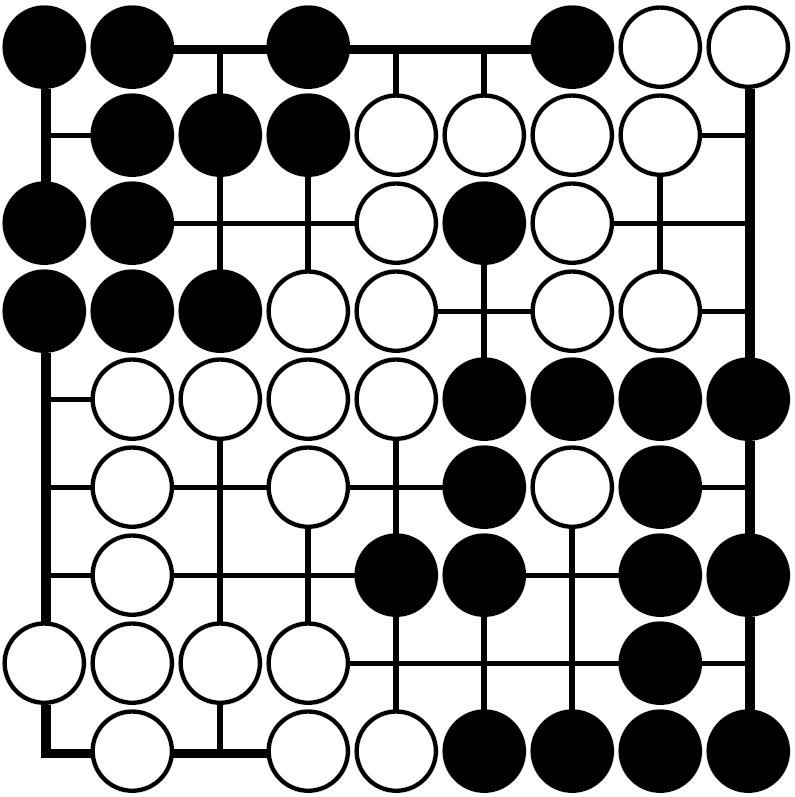
\includegraphics[width=.4\textwidth]{../img/late_endgame_Go_position_suited_for_exact_analysis.png}
  \captionWithCite{An~immortal wall enabling an exact analysis during late endgame}{Muller1995computer}
  \label{fig:immortal-wall}
\end{figure}
No move can have any influence across these ``immortal'' walls and significant parts of~the board definitely belong to one of the players.
The connected components of~remaining stones define local subgames independent from each other.

In the opening and midgame, only approximate partitioning can be available.
In the endgame, conversely, the partition gets more precise:
the status of~all big groups has been settled, and the outlines of~territories are clear.
If each local game is simple enough to~analyze completely (such as in Figure~\ref{fig:immortal-wall}), combinatorial game theory can compute an~optimal move for the full board position.
(\cite{Muller1995computer})

This is the general procedure of~(\cite{Muller1995computer}) for playing Go as a~sum of~local games:
\begin{enumerate}
  \item Board partition: find safe blocks, safe territories, and local areas.
  \item Generate local game trees in each area.
  \item Evaluate local terminal positions.
  \item Transform local game trees into mathematical games (and simplify games).
  \item Find an optimal move in the (combinatorial game theory) sum-game and play it.
\end{enumerate}
\Mueller{} proposes heuristic algorithms for playing the entire game, and exact algorithms for late endgame positions.

Undoubtedly, the task of~solving endgames in 1995 (at the age of Computer Go's infancy) already played a~vital role.

\section{Combinatorial Game Theory for the Game of~Go}

\epigraph{
  [$\dots$]
  You get surreal numbers by~playing games.

  I used to feel guilty in Cambridge that I spent all day playing games, while I was supposed to be doing mathematics.
  Then, when I discovered surreal numbers, I realized that playing games IS math.
}{John Horton Conway}
\Mueller{} suggests to replace the ``standard model'' of~computer Go by a~sum-game model.

Here follows some of~the general benefits and problems of~the sum-game model for computer Go as listed in~(\cite{Muller1995computer}):

\medskip

\underline{Benefits}
\begin{itemize}[+]
  \item suitability to the knowledge and style of~Go programs at that time:
    local fighting, surrounding territories$\dots$
  \item the reuse of~local game analysis for higher quality game-play
  \item simplification of~move generation and position evaluation
  \item translation of~Go terms into the theory, without any need for~separate programming
  \item evaluation of~the opponent's endgame moves
  \item assessment of~sufficiently good moves even with a~\emph{reduced} local game database
  \item position's game-theoretic value computed long before the end
  \item opportunities for parallelism:
    independent local searches, evaluation and operations on mathematical games$\dots$
  \item perfect computer play in~late endgame
\end{itemize}

\underline{Obstacles}
\begin{itemize}[-]
  \item required accurate board partition and recognition of~dependencies
  \item the common issues of~selective search:
    misleading evaluation due to missing crucial moves in~complicated games
  \item the lack of~long-range full-board planning:
    ``This is probably not a~big issue until programs reach amateur Dan or even professional level.''%
    \footnote{For an~update on the situation today, see Chapter~\ref{ch:AlphaGo}.}
\end{itemize}

The strict endgame analysis of~(\cite{Muller1995computer}) is additionally impossible, when one of~the following \underline{limitations} is met:
\begin{itemize}[-]
  \item \textbf{partition:}
    There is insufficient amount of~blocks that can be proven safe.
    Some of~the areas are hence too large for~the complete search.
  \item \textbf{summation:}
    No~move with dominating incentive exists, and both summing and partial search would take too long.
  \item \textbf{Ko:}
    Combinatorial game theory relies on the independence of~local subgames.
    In the case of~Ko, the independence is broken:
    a~locally bad move may be globally best if it serves as a~Ko threat (recall Section~\ref{sec:Go}).
    \Mueller{} mentions in~1995 there was ongoing research to generalize the theory for handling Kos.
  \item \textbf{Unneccessary complexity in ``straightforward'' situations:}
    In cases where the focus of~play is straightforward (i.e. only one local situation is relevant), combinatorial game theory introduces additional complexity.
    Namely, CGT investigates moves for~both players in~this and every other position.
\end{itemize}

\section{Board Partition and Subgame Dependencies}
\epigraph{
  Independence?
  That's middle class blasphemy.
  We are all dependent on~one another, every soul of~us on Earth. 
}{George Bernard Shaw}
In addition, (\cite{Muller1995computer}) mentions several further obstacles of~the sum-game model, caused by~the heuristic board partition:

\begin{itemize}[-]
  \item the impossibility of a~perfect, precise split:
    During the opening or~midgame, there are almost no surrounded spaces, and moreover, the surrounding stones would not be invulnerable yet.
    Heuristics is needed for board partition to split the imperfectly surrounded areas.

  \item the infeasibility of~exhaustive search in still large subgames:
    The program is obliged to give a~move in a~few seconds or minutes.
    However, there still remain areas intractable for an~exhaustive search.

    In such subgames, \Mueller{} employs \emph{selective search} method.
    He limits the number of~generated moves and stops the search before reaching a~terminal position.
    For each local game, nodes to expand need to be decided and \emph{expert modules for search and evaluation} need to be selected.
    A~post-processing stage handles detected dependencies between games.

  \item the dependencies between the resulting subgames, which arise with the previously mentioned heuristics:
    The effect of~such dependencies differs widely:
    often it is so small that independence is a~useful approximation.
    In cases when a~move works as a~\emph{double threat} however, dependency analysis is crucial.

    Trivial strategies to overcome dependencies involve:
    \begin{itemize}
      \item ignoring the dependency, as if the games were independent,
      \item proving that the dependency does not affect the value of~the sum, or play of~the sum game,
      \item merging mutually dependent local games, then re-search the combined game, possibly using previously generated information on single games,
      \item analyzing the interaction between local games, then use a~specialized theory to compute the joint game value.
    \end{itemize}
\end{itemize}

Hence, the sum game model makes the best sense during the endgame part.
This general principle is as well applicable in poker:
we wait until the late stage of~the game, when it has greater impact to refine and re-solve the reached endgames.

\section{Local Search and Evaluation in the Endgame}
\epigraph{
  True genius resides in~the capacity for~evaluation of~uncertain, hazardous, and conflicting information. 
}{Winston Churchill}
Once the board is partitioned, the algorithm of~(\cite{Muller1995computer}) for converting a~Go endgame into a~combinatorial game follows these steps:
\begin{enumerate}
  \item Generate local game trees:
    all legal moves are generated from point of~both players, with exceptions~of:
    \begin{enumerate}[(a)]
      \item \emph{pruning rules}%
        \footnote{Compare with \emph{policy networks} of~AlphaGo in Chapter~\ref{ch:AlphaGo}.},
        e.g. pruning dominated subgame trees:
        the evaluation of~nodes allows for pruning moves dominated by other moves.
        Moves with a~dominating alternative are labelled as~\emph{locally bad moves}.

      \item \emph{termination rules} for static evaluation of a~position, without further tree expansion%
        \footnote{Compare with \emph{value network} of~AlphaGo in Chapter~\ref{ch:AlphaGo}.}
    \end{enumerate}

  \item Score local terminal positions:
    \begin{enumerate}[(a)]
      \item \emph{scoring}%
        \footnote{See Section~\ref{sec:Go}.}
        comes in two widely-accepted flavors, namely
        \begin{enumerate}[$\diamondsuit$]
          \item Chinese variant, which counts stones and empty points belonging to either color,
          \item Japanese variant, which counts territory and prisoners.
        \end{enumerate}
        Both variants have straightforward implementation because safe stones, dead stones, territories and neutral points are known exactly in~the endgame.

      \item \emph{terminal positions} can be recognized by
        \begin{enumerate}[$\diamondsuit$]
          \item no more legal moves,
          \item no more good moves,
          \item the value of~position already known from the transposition table, pattern, or local position database.
        \end{enumerate}
        A~position is additionally considered terminal, once we can ascertain its value from another source.
        Such a~value can be any value in~the sense of~mathematical games.

        Non-terminal positions may have a~constant value as well, if the outcome is the same no matter who plays first, but this has to be proven using search.
    \end{enumerate}

  \item Evaluate local games as mathematical games.
    Explicitly, evaluate terminal positions, and back up the values in~the tree, resulting in a~mathematical-game evaluation of~each node.

    Even though the program reaches a~solved position, (\cite{Muller1995computer}) notes that a~``suicidal'' opponent may later cause great troubles, by endangering his immortal stones.
    Such an~act would violate the assumptions on~board partitioning and give rise to~new unexpected positions with rather complicated optimal play.

  \item Select an~option in the resulting (abstract) sum-game.
  \item Translate the chosen option in~the abstract game into a~corresponding move in~Go.
    This move is taken as~the first move with sufficient \emph{incentive} (recall Section~\ref{sec:CGT}).
\end{enumerate}

\begin{figure}[H]
  \centering
  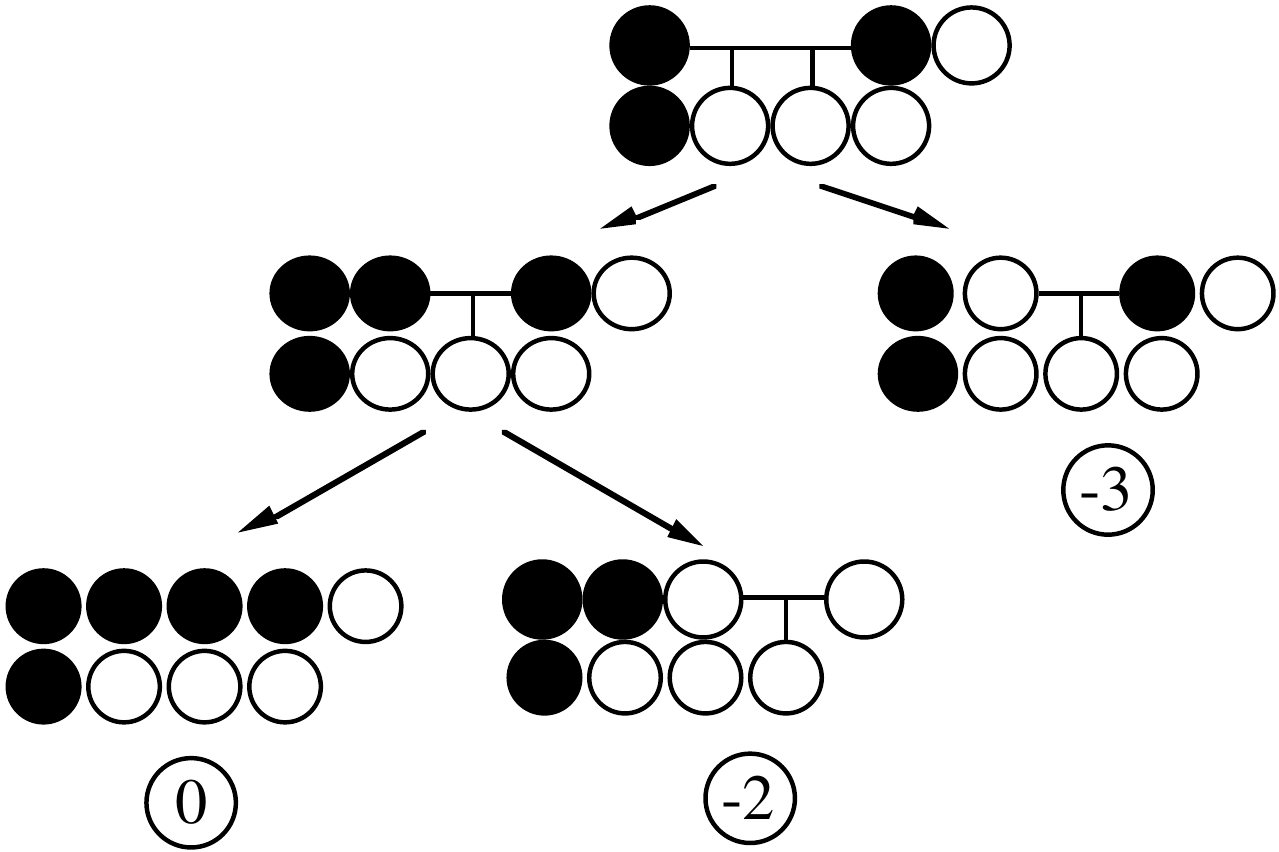
\includegraphics[width=.5\textwidth]{../img/Go_search_tree.png}
  \captionWithCite{Local game tree with evaluation of terminal nodes}{Muller1995computer}
\end{figure}

\section{Storing Search Results into Database}
\epigraph{
  I'm blessed with very fast memorization skills, so I don't have to read it too far in advance.
}{Jaimie Alexander}
Search and analysis produce the complete description of possible endgame plays, facilitating the perfect strategy.
The results are stored in a~\emph{database of~local positions}.
Local subgames during a~live play are then matched one-to-one to a~set of~database positions.
The value of a~full board position is the sum of~local position values and an~algorithm for sum-game evaluation selects the best available response.

A~version with lower memory requirements is implemented as well.
This is achieved by~saving only a~selection of~positions, and in~case the subgame is missing in the database, re-doing the search.

An~important question is what to store.
Table~\ref{tab:db-loc-games} lists some possible answers:
\begin{table}[!htbp]
  \centering
  \begin{tabular}{ |p{.45\textwidth}|p{.48\textwidth}| } 
    \hline
    \textbf{Type of database} & \textbf{Content} \\
    \hline
    Full                            & $\dots$every position discovered during exhaustive search \\
    Color-complete (Black or White) & $\dots$every position reachable by~non-dominated moves of~the color and arbitrary opponent's moves (pruned bad moves of~the color) \\
    Optimal                         & $\dots$at~least one position corresponding to~every non-dominated option of~every reachable position (guaranteed optimal play from every position in~database) \\
    Sufficiently good               & $\dots$guaranteed optimal score from a~starting position (might fail to exploit some opponent mistakes) \\
    \hline
  \end{tabular}
  \captionWithCite{Possible database variants of~local games}{Muller1995computer}
  \label{tab:db-loc-games}
\end{table}

One needs to make a~trade-off between re-computation time and storage space.
A~sensible solution is to~store only complicated moves in~the database, and re-calculate the rest when necessary.
It is a~good idea to save only the information whether a~move is locally good or bad, but discard \emph{refutations}\footnotemark.
\footnotetext{the trees proving that bad moves are inferior}
Such a~type of~database is robust against a~good opponent;
however, it suffers from a~play of a~locally bad opponent.
This~rare situation would call for the re-computation of~a~subtree in order to find a~refutation.

The number of~possible moves in an $n$-point area is approximately $2n$ ($n$ for each player), and such a~play generates a $n-1$ point area.
Whence, the size of~the game tree is approximately $2n\cdot2(n-1)\cdot \ldots \cdot2 = 2^n n!$ nodes.
Such a~combinatorial explosion makes even fairly small endgames prohibitively expensive.
\Mueller{} overcomes this hardness with a~transposition table.
A~\emph{transposition table} detects identical board positions, reducing the size of~the search space from $\approx 2^n n!$ to $3^n$ states (see the comparison in Table~\ref{tab:reduction-transp-tab})
\begin{table}[!htbp]
  \centering
  \begin{tabular}{ |rrr| }
    \hline
    \textbf{$n$} & \textbf{$2^nn!$} & \textbf{$3^n$} \\
    \hline
    1	&	2	&	3 \\ 
    2	&	8	&	9 \\ 
    3	&	48	&	27 \\ 
    4	&	384	&	81 \\ 
    5	&	3840	&	243 \\ 
    6	&	46080	&	729 \\ 
    7	&	645120	&	2187 \\ 
    8	&	10321920	&	6561 \\ 
    9	&	185794560	&	19683 \\ 
    10	&	3715891200	&	59049 \\ 
    \hline
  \end{tabular}
  \caption{Reduction of search space by transposition table}
  \label{tab:reduction-transp-tab}
\end{table}

\section{Pattern Learning}
{
  \setlength{\epigraphwidth}{0.55\textwidth}
  \epigraph{To understand is to~perceive patterns.}
  {Isaiah Berlin}
  \epigraph{When patterns are broken, new worlds emerge.}
  {Tuli Kupferberg}
}%
Pattern recognition is one of~the key components of~AlphaGo (see Chapter~\ref{ch:AlphaGo}).
Arguably, the program's success might be partially attributed to learning Go patterns from human expert plays.

For comparison, (\cite{Muller1995computer}) hails computer Go as \emph{a~vehicle for research in~visual perception, machine learning and neural networks} (based on~\cite{Wilcox79}; \cite{Enderton1991golem}; \cite{Stoutamire1991machine}; \cite{Schraudolph1994temporal}).

Being introduced just and only to~Go rules, learning programs can typically pick up basic Go principles, such as saving a~stone from capture, and familiarize themselves with~low-level game concepts.
However, these concepts and principles have already been integrated into~other far superior \emph{expert-based programs}.
Neural networks are therefore more adapt at~playing locally good shapes, but possess no~idea when to play it.%
\footnote{This assertion especially has changed thanks to~AlphaGo.}
These systems are vulnerable to other Go agents with better knowledge of~tactics.

In the end, (\cite{Muller1995computer}) suggests \emph{pattern matching} as a~promising means for the significant advancement of~computer Go.

\section{Contributions of~Combinatorial Game Theory to Go Endgames}
\epigraph{
  You can retire from a~job, but don't ever retire from making extremely meaningful contributions in~life.
}{Stephen Covey}
\Mueller's doctoral thesis acclaims following contributions to computer science:
\begin{itemize}
  \item ``Scientists are fascinated by problems which can be stated simply, yet are hard to solve.
    Computer Go is a~prime example.
    We have brought the divide-and-conquer approach, a~fundamental paradigm of~computer science, to bear on computer Go.''

  \item ``The application of a~sophisticated mathematical theory to computer Go provides an~example of~algorithms for a~nontrivial decomposition of a~complex problem.''
\end{itemize}
and following contributions to computer Go:
\begin{itemize}
  \item ``We have implemented a~\emph{late endgame player}, a~niche where program play surpasses human play in both speed and exactness.
    We did this by applying concepts from combinatorial game theory to Go.
    The program plays a~wide variety of`late endgame positions perfectly.''

  \item ``We have developed algorithms for board partition and dependency analysis.''
\end{itemize}
Hence, the work employs a~technique of~applying an~elaborate mathematical theory (of~combinatorial game theory) to deal with the endgame phase.
In particular, CGT is used to ``connect'' individual relevant subgames, which may be solved independently.

As we will see later, the situation in the case of~Poker is slightly more delicate:
the imperfect-information property prevents us from using an~immediate divide-and-conquer approach.
Instead, we will \emph{augment} the information by saturating it with additional game states (see Chapter~\todo).

\note{
  \label{note:CGTvsAlphaGo}
  It is also interesting to compare the method of~(\cite{Muller1995computer}) with the modern approach of~\emph{AlphaGo}:
  the ad-hoc Go-specific knowledge is replaced with general-learning neural networks and the probabilistic \emph{Monte Carlo Tree Search} algorithm.
  Such a~combination has the capability to surpass professional human players at the highest ranks.
  What's more, this solution can be adapted to other games without substantial modifications.
  With data, the system can be trained without any need to imbue it with game-specific knowledge.
  Follow Chapter~\ref{ch:AlphaGo} for more details.
}

\chapter{Go Endgames Using Neural Networks}
\label{ch:AlphaGo}
\epigraph{
  Creativity involves breaking out of established patterns in order to look at things in a different way.
}{Edward de Bono}
As of~today, over 20 years have passed since \Mueller's work.
\emph{DeepMind}, a~London-based AI start-up recently acquired by Google, has developed the strongest computer Go program so far:
\emph{AlphaGo}.

\note{
  This chapter is based on~the article ``Mastering the game of Go with deep neural networks and tree search''~(\cite{Silver2016mastering}), which documents the internals of~AlphaGo.

  For more details, also consult my presentations on AlphaGo given at:
\begin{itemize}
  \item Spring School of Combinatorics 2016 (Charles University in~Prague): \\
    \href{http://www.slideshare.net/KarelHa1/mastering-the-game-of-go-with-deep-neural-networks-and-tree-search-presentation}
    {\tt http://www.slideshare.net/KarelHa1/mastering-the\\-game-of-go-with-deep-neural-networks-and-tree\\-search-presentation}

  \item Optimization Seminar (Charles University in~Prague) \\
    \href{http://www.slideshare.net/KarelHa1/alphago-mastering-the-game-of-go-with-deep-neural-networks-and-tree-search}
    {\tt http://www.slideshare.net/KarelHa1/alphago\\-mastering-the-game-of-go-with-deep-neural\\-networks-and-tree-search}

  \item Distributed Computing group (ETH \Zurich) \\
    \href{http://www.slideshare.net/KarelHa1/alphago-for-disco-group-of-eth-zurich}
    {\tt http://www.slideshare.net/KarelHa1/alphago\\-for-disco-group-of-eth-zurich}
\end{itemize}
}

\section{Game-Tree Search}
\epigraph{
  There are more possible positions in~Go than there are atoms in~the universe.
  That makes Go a~googol [$10^{100}$] times more complex than chess.
}{\href{https://deepmind.com/alpha-go.html}{Google DeepMind}}
Optimal value~$v^*(s)$ determines the~outcome of~the game from every board position $s$ under perfect play by~all players.
This value can be computed by~recursively traversing the~search tree containing approximately $b^d$ possible sequences of moves, where $b$ is the breadth of~game (number of legal moves per position) and $d$ is its depth (game length).

In~the case of~chess, that is $b \approx 35$ and $d \approx 80$, whereas Go has $b \approx 250$ and $d \approx 150$.
This amounts to a~terrifying overnumerousness: there are more Go positions than atoms in the observable Universe.
Therefore, exhaustive search is deemed intractable.

How to handle the size~of the game tree?
\begin{itemize}
  \item For the breadth, we train \emph{a~neural network to~select} moves.
  \item For the depth, we train \emph{a~neural network to~evaluate} the current position.
  \item For the tree traverse, we use \emph{Monte Carlo tree search} method.
\end{itemize}

\textbf{Monte Carlo tree search} (MCTS) is a~Monte Carlo heuristic of~the classical tree search.
However, instead of traversing the entire game tree, the MCTS selects the~most promising moves, expanding the search tree based on~random sampling.

In~each iteration, the game is played-out to~the very end by~choosing moves at~random.
The final outcome of~each playout is then used to~weight the nodes in~the game tree accordingly.
Thus, better nodes are more likely to be chosen in future playouts.

\begin{figure}[H]
  \centering
  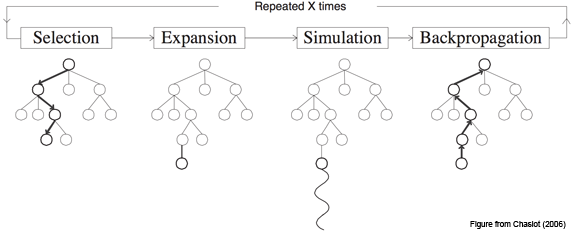
\includegraphics[width=.6\textwidth]{../img/MCTS.png}
  \caption{The scheme of~MCTS}
  \label{fig:MCTS}
\end{figure}

\section{Neural networks}
\epigraph{
  Your brain does not manufacture thoughts.
  Your thoughts shape neural networks.
}{Deepak Chopra}
Inspired by biological neural networks, an~artificial neural network (ANN, see Figure~\ref{fig:shallow-neural-network}) is a~network of~interconnected nodes that make up a~model.
\begin{figure}[H]
  \centering
  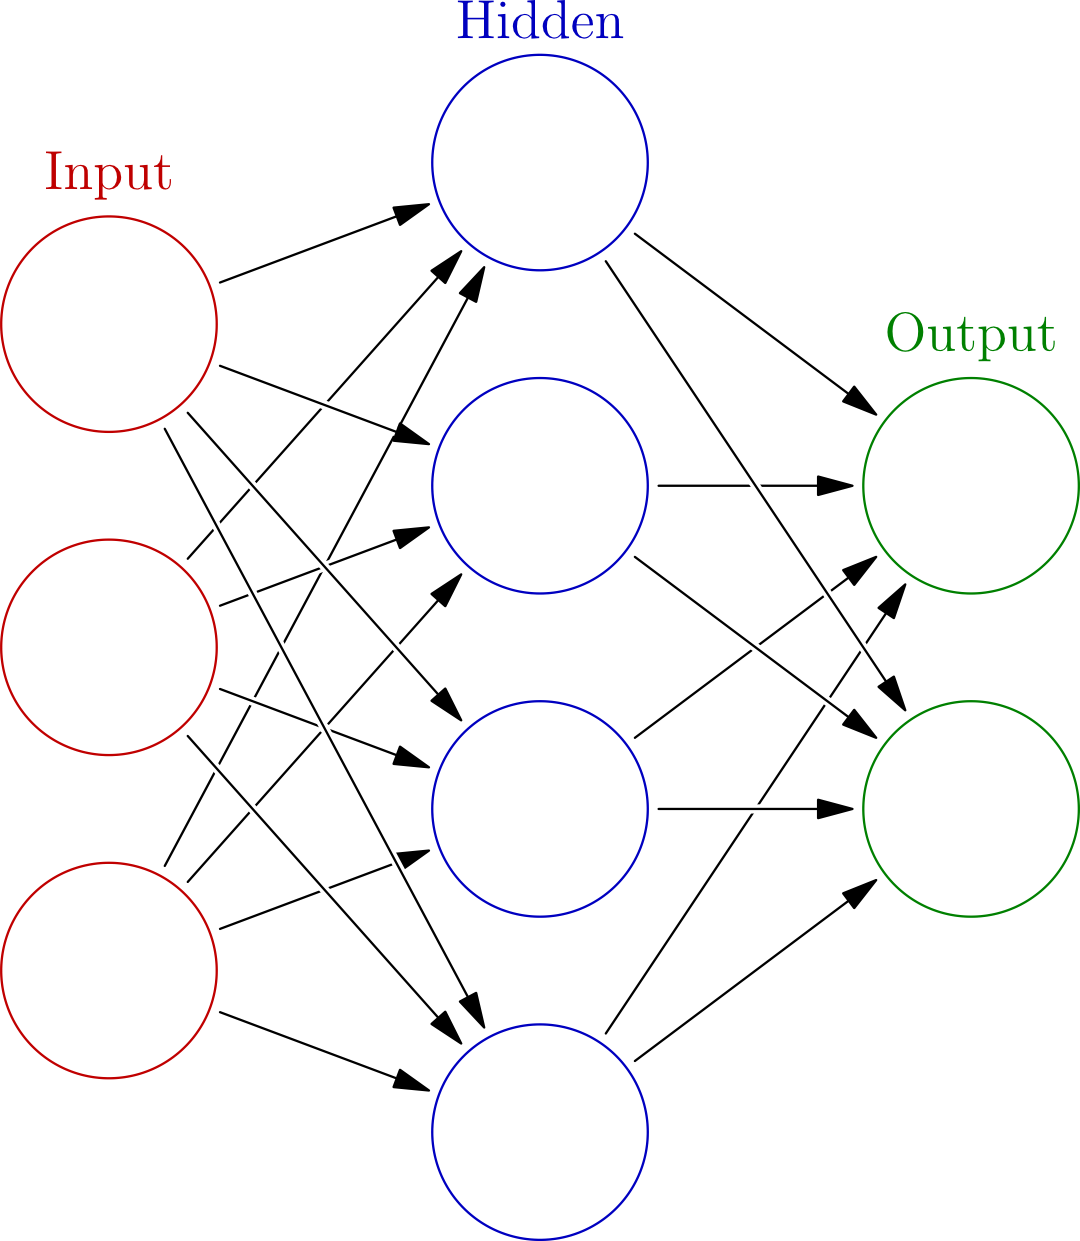
\includegraphics[height=.2\textheight]{../img/colored_neural_network.png}
  \caption{A~shallow neural network with 3 layers}
  \label{fig:shallow-neural-network}
\end{figure}
ANNs can be defined as~statistical learning models that are used to approximate functions which depend on a~large number of~inputs.
Neural networks are typically used when the volume of~inputs is far too large for~standard machine learning approaches.

\textbf{Convolutional neural network} (CNN) is a~neural network suitable for high-dimensional inputs (e.g. a~large number of~pixels in an~image).
CNNs are frequently used in~computer vision (for identifying objects in an~image, for face detection in~photos etc.).
They are invariant to expectable transformations of~input, such as translations of~objects in~a~picture or changes in~illumination.

\textbf{Deep neural network} (DNN) is a~neural network with many hidden layers.
It can model complex non-linear relationships, e.g. in~speech, in~images, in~videos or in~board positions of~Go.

\section{Pipeline of Neural Networks}
\epigraph{
  Pattern recognition and association make up the core of~our thought.
  These activities involve millions of~operations carried out in~parallel, outside the field of~our consciousness.

  If AI appeared to hit a~brick wall after a~few quick victories, it did so owing to~its inability to~emulate these processes.
}{Daniel Crevier}
AlphaGo employs two kinds of deep convolutional neural networks---a~\emph{policy network} (for move selection) and a~\emph{value network} (for board evaluation).
\begin{figure}[H]
  \centering
  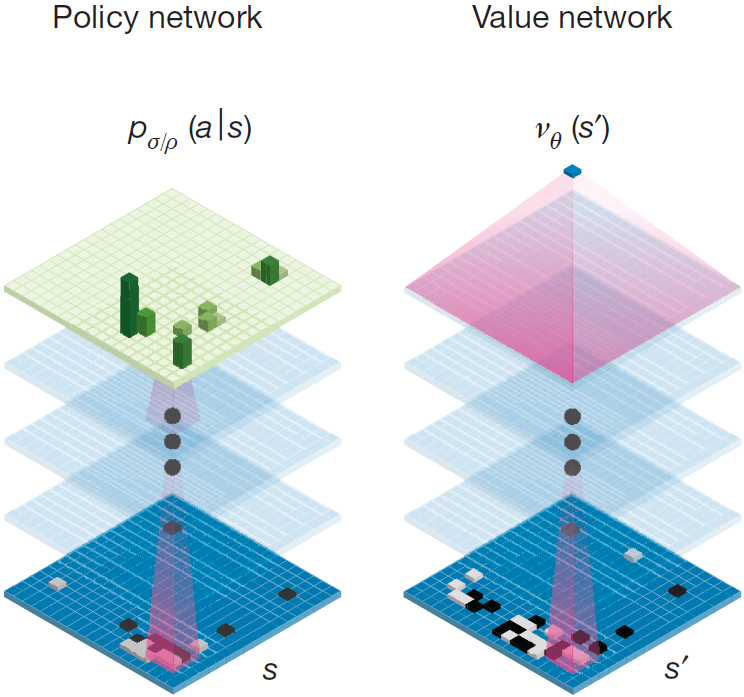
\includegraphics[width=.5\textwidth]{../img/policy_and_value_network.png}
  \captionWithCite{Comparison between policy and value network}{Silver2016mastering}
  \label{fig:policy_vs_value_nets}
\end{figure}

In the following Figure~\ref{fig:neural_nets_pipeline}, we can view the whole training process of~AlphaGo's neural networks.
\begin{figure}[H]
  \centering
  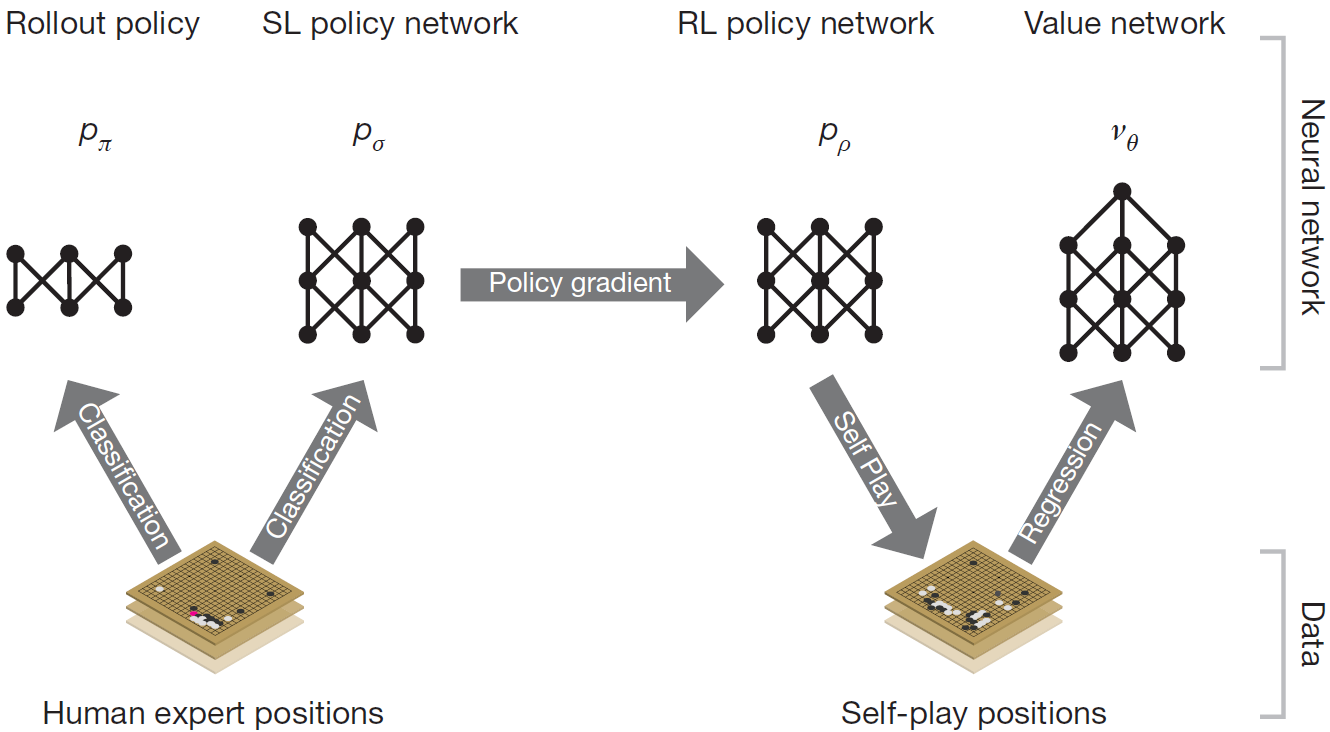
\includegraphics[width=.7\textwidth]{../img/neural_nets_pipeline.png}
  \captionWithCite{Training the neural networks of~AlphaGo: the~pipeline~and~the~architecture}{Silver2016mastering}
  \label{fig:neural_nets_pipeline}
\end{figure}

\textbf{Rollout policy} $p_\pi$ is a~CNN rapidly sampling actions during a~\emph{rollout} (a~fast-forward simulation from a~position to the end of~the game).
It predicts expert human moves much faster but less accurately than $p_\sigma$ (see below).
The output is a~probability distribution over all moves.

\textbf{Policy network} is a~CNN selecting moves.
It addresses the problem of the game-tree breadth.
There are two flavors of~these networks:
\begin{itemize}
  \item \textbf{SL policy network} $p_\sigma$ is trained by \underline{s}upervised \underline{l}earning to predict expert human moves.
  \item \textbf{RL policy network} $p_\rho$ is trained by \underline{r}einforcement \underline{l}earning to win in the~games of~self-play.
\end{itemize}

\textbf{Value network} $v_\theta$ is a~CNN evaluating board positions, so as to address the problem of the game-tree depth.
It is trained by regression to predict the outcome in~positions of~the self-played games.

\section{Main Algorithm of~AlphaGo}

Finally, the neural networks are combined with MCTS into the main algorithm.

During the play, AlphaGo simulates up to 100 possible continuations per each move by selecting the most promising actions and following them.
This way, it descends the game-tree down to a~depth given by a~parameter.
At that point, leaf nodes are evaluated in two ways:
\begin{enumerate}[(1)]
  \item using the dedicated value network $v_\theta$,
  \item simulating the self-play until the terminal positions, using the fast rollout policy $p_\pi$.
\end{enumerate}
The two are mixed into the final value of~the leaf node.

Once every simulation of a~single round is finished, all new values are backpropagated to the root, thus updating necessary variables on the way up.

For more details, consult (\cite{Silver2016mastering}) or the before-mentioned presentations.

\note{
  Main algorithm demonstrates the connection to \emph{our theme of~endgames}:
  the simulations may be viewed as ``solving endgames''.
  In particular, the $p_\pi$ rollouts somehow remind of~exhaustive search for the game value during the late stage of~the play.
  In this sense, the approaches of~AlphaGo and endgame computation bear a~striking similarity.

  On the other hand, AlphaGo performs the same simulation algorithm during the whole game:
  from an~empty board until the final move.
  Therefore, it would be imprecise to talk about ``endgame'' here.
}

\section{Playing Strength}

In order to assess the playing strength of~AlphaGo, DeepMind has organized an~internal tournament between different other Go programs,%
\footnote{\emph{CrazyStone} and \emph{Zen} are the strongest commercial programs, whereas \emph{Pachi} and \emph{Fuego} are strongest among the open-source ones.}
as well as a~duel of~AlphaGo against the European Go Champion Fan Hui.
Figure~\ref{fig:Go-tournament} displays the outcome of the tournament:

\begin{quotation} \noindent
  Each program used approximately 5 s computation time per move.
  To provide a~greater challenge to AlphaGo, some programs (pale upper bars) were given four handicap stones (that is, free moves at~the start of~every game) against all opponents.
  Programs were evaluated on an Elo scale: a~230 point gap corresponds to a~79\% probability of winning, which roughly corresponds to one amateur dan rank advantage on KGS;
  an~approximate correspondence to human ranks is also shown, horizontal lines show KGS ranks achieved online by that program.
  Games against the human European champion Fan Hui were also included;
  these games used longer time controls.
  95\% confidence intervals are shown.~(\cite{Silver2016mastering})
\end{quotation}

\begin{figure}[H]
  \centering
  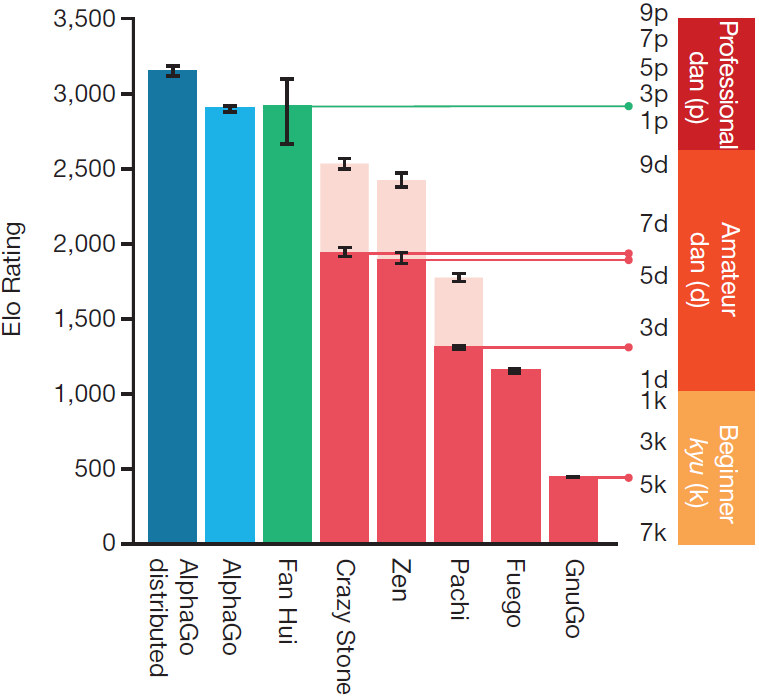
\includegraphics[width=.5\textwidth]{../img/results_of_tournament.png}
  \captionWithCite{Tournament with other programs and Fan Hui}{Silver2016mastering}
  \label{fig:Go-tournament}
\end{figure}

Here is an~official report provided by Google DeepMind%
\footnote{\href{https://deepmind.com/alpha-go.html}{https://deepmind.com/alpha-go.html}}
about AlphaGo's matches against human professionals:
\begin{quotation} \noindent
  After our program AlphaGo won 5--0 in a~formal match on~October 2015, against the reigning 3-times European Champion, Fan Hui, becoming the first program to ever beat a~professional Go player in an~even game;
  AlphaGo then went on to complete its ultimate challenge.

  In March 2016 AlphaGo won 4--1 against the legendary Lee Sedol, the top Go player in the world over the past decade.
  The matches were held at the Four Seasons Hotel, Seoul, South Korea on March 9\textsuperscript{th}, 10\textsuperscript{th}, 12\textsuperscript{th}, 13\textsuperscript{th} and 15\textsuperscript{th} and livestreamed on DeepMind’s YouTube channel as well as broadcast on TV throughout Asia through Korea’s Baduk TV, as well as in China, Japan, and elsewhere.

  They were played under Chinese rules with a~komi of~$7.5$ (the compensation points the player who goes second receives at~the end of~the match).
  Each player received two hours per match with three lots of 60-second byoyomi (countdown periods after they have finished their allotted time).
\end{quotation}

Following from this, computers seem to have reached the ``superhuman'' level of~expertise and they now appear to be superior to humans in~the game of~Go.

%%%%%%%%%%%%%%%

%%% Part II %%%
\part{Imperfectness of~Imperfect-Information Endgames}
\chapter{Setting the Scene for Imperfect Information}
\epigraph{
  Intelligence is a~game of~imperfect information.
  We can guess our opponent's moves, but we can't be sure until the game is over.
}{Khalid Muhammad}

\section{Games with Turns}

\subsection{Extensive Form}
\label{ssec:extensive-form}

An \emph{extensive-form game} consists of

\begin{itemize}
  \item a finite set of \emph{players} $P$,
  \item a finite set $H$ of all possible \emph{histories},
    \begin{itemize}
      \item Each history consists of individual \emph{actions}.
      \item $h \sqsubseteq h'$ denotes that history~$h$ is a~prefix of $h'$.
      \item $\emptyset \in H$ and $h' \in H \land h \sqsubseteq h' \implies h \in H$
      \item Set $Z \subseteq H$ is the set of \emph{terminal histories}, i.e. histories that are not prefixes of any other histories.
    \end{itemize}
  \item the set of available actions $A(h) = \braces{a: (h, a) \in H}$ for every node $h \in H \setminus Z$,
  \item a~function $P()$ assigning an~\emph{acting player} to each $h \in H \setminus Z$.
    The acting players are taken from the set $P \cup \braces{c}$, where $c$ is the \textbf{c}hance player (e.~g. a~dice, the card dealer, the nature etc.).
    Thus, $P(h) \in P \cup \braces{c}$ for any $h \in H \setminus Z$.
  \item a~function $f_c$ determining the probability measure over actions $A(h)$ for nodes $h$ with $p(h) = c$, the nodes of the chance player.
  \item The partition $\I_i$ of nodes $\braces{h \in H: p(h) = i}$ is called the \emph{information partition} of player~$i$.
    Its element $I \in \I_i$ is an \emph{information set} of player~$i$ and $I(h) \in \I_i$ (with $p(h) = i$) denotes the information set containing $h$.

    An information set represents grouping of histories that are indistinguishable from $i$'s point of view.
    In the game of poker, for example, this might be because of hidden cards of opponents.
  \item a \emph{utility function} $u_i\colon Z \goto \R$,
\end{itemize}

There are further notions related to any extensive-form game:

\begin{itemize}
  \item \emph{Strategy}~$\sigma_i$ of (non-chance) player~$i$ determines a~probability distribution over $A(I)$ at every $I \in \I_i$.
    Thus $\pi ^\sigma (I, a)$ is the probability of action $a$ at the information set~$I$.
    $\Sigma_i$ denotes the set of all possible strategies for player~$i$.
  \item A~\emph{strategy profile} is a~vector of all (non-chance) players' strategies denoted by $\sigma = (\sigma_1, \sigma_2, \ldots, \sigma_ {\abs{P}})$.
    The set of all such possible strategy profiles is denoted by $\Sigma$.
    Hence, it is the Cartesian product $\Sigma = \prod\limits _{i \in P} \Sigma_i$.
  \item We use the Greek letter $\pi$ to evaluate the probability corresponding to a~profile~$\sigma$:
    \[\pi ^\sigma(h) = \prod _{i \in P \cup \braces{c}} \pi _i ^\sigma (h)\]
    
  \item The probability $\pi _{-i} ^\sigma (h)$ (or sometimes just briefly $\pi _{-i} (h)$) is the product of~all players' contribution, except for the one of player~$i$:
    \[\pi _{-i} ^\sigma(h) = \prod _{j \in P \setminus \braces{i} \cup \braces{c}} \pi _j ^\sigma (h)\]
    
  \item $\sigma | _{I \goto a}$ denotes the strategy identical to $\sigma$ with the only one exception:
    the action~$a$ is always played at the information set~$I$.
  \item Given the strategic profile $\sigma$, the \emph{expected utility}~$u_i (\sigma)$ for player~$i$ is defined as:
    \[ u_i (\sigma) = \sum _{z \in Z} \pi ^\sigma (z) u_i(z)\]

  \item A~\emph{best response} $BR _i (\sigma _{-i})$ (or briefly $BR _i (\sigma)$) of player $i$ for given $\sigma _{-p}$ is such a~strategy $\sigma _i \in \Sigma _i$ that maximizes player's expected utility against others:
    \[ u_i (\sigma) = \max _{\sigma'_i \in \Sigma_i} u_i ((\sigma'_i, \sigma_{-i})) \]

  \item A~\emph{Nash equilibrium} (in the context of extensive-form games) is a~strategy profile $\sigma$ such that no player~$i \in P$ has any incentive to deviate from his strategy.
    In other words, all players are playing best responses against each other:
    \[ \forall i \in P\colon u_i (\sigma) = \max _{\sigma'_i \in \Sigma_i} u_i ((\sigma'_i, \sigma_{-i})) \]

  \item The \emph{counterfactual value} $v _i ^\sigma (I)$ is the expected utility provided that the information set $I$ is reached and all players play according to strategy $\sigma$ with exception of player~$i$, who plays to reach $I$:
    \[ v _i ^\sigma (I) = \sum\limits _{h \in I, \; h' \in Z}
      \frac
      {\pi _{-i} ^\sigma(h) \pi ^\sigma(h,h') u_i(h')}
      {\pi _{-i} ^\sigma (I)} \]

  \item A~\emph{counterfactual best response} $CBR _i (\sigma _{-i})$ (or briefly $CBR _i (\sigma)$) of player~$i$ is a~strategy maximizing the counterfactual value at each information set $I \in \I _i$:
    \[ \pi ^\sigma (I, a) \geq 0
      \; \Longleftrightarrow \;
      v _i ^\sigma (I, a) = \max _{a' \in A(I)} v _i ^\sigma (I, a') \]

    Note that $CBR _i (\sigma)$ is always a best response $BR _i (\sigma)$, but the reverse implication does not need to hold:
    a~best response $\sigma$ can select an~arbitrary action in an~unreachable information set $I$ (the one where $\pi ^\sigma (I) = 0$).
    Such best responses are in general not counterfactual best responses.

  \item For the sake of notation's simplicity, we will define \emph{counterfactual best response value} as the counterfactual value for the strategy, where player $i$ plays according $CBR _i (\sigma _{-i})$ rather than the original $\sigma$.
    Formally, it is
    \[ CBV _i ^\sigma (I) = v _i ^{(\sigma _{-i}, CBR _i (\sigma _{-i} ))} (I) \]

\end{itemize}

There may be various properties for extensive-form games:

\begin{itemize}
  \item being \emph{two-player}
  \item having \emph{perfect recall}: any two states from the same information set $I \in \I _i$ share the same history of past actions and player $i$'s information sets.

    In other words, at any stage of the game no player can forget what happened so far:
    neither actions taken nor the information sets reached.
  \item being \emph{zero-sum}: For any $\sigma \in \Sigma$ we have $\sum _{i \in P} u _i (\sigma) = 0$.
\end{itemize}

\subsection{Sequence Form}

\section{Methods of~Solution}

\subsection{Linear Programming}
{
  \setlength{\epigraphwidth}{0.65\textwidth}
  \epigraph{
    If you optimize everything, you will always be unhappy.
  }{Donald Ervin Knuth}
}

\subsection{Learning}
{
  \setlength{\epigraphwidth}{0.65\textwidth}
  \epigraph{
    Perfecting oneself is as~much unlearning as~it is learning.
  }{Edsger Dijkstra}
}

\section{Subgames (Endgames)}

So far, the information sets have grouped only those states where the player was the acting player.
For the purposes of the subgame, it is also necessary to include the states that are indistinguishable from the point of view of other players.
Therefore, we define the \emph{augmented information sets} (\cite{BurchJohansonBowling13}):

\begin{itemize}
  \item For any player $i \in P$, let $H_i(h)$ be the sequence of player $i$'s information sets reached by player $i$ on the path to $h$, and the actions taken by player~$i$.
  \item An~\emph{augmented information set} $I_i(h)$ is defined by the following characterization:
    for any two states $h, h' \in H$, we have that 
    \[ I_i (h) = I_i (h') \; \Longleftrightarrow \; H_i (h) = H_i (h') \]
\end{itemize}

At this point, we may finally define the notion of a~\emph{subgame}:

\begin{itemize}
  \item An~(imperfect information) \emph{subgame} is a~forest of trees, closed under both the descendant relation and membership within augmented information sets for any player (\cite{BurchJohansonBowling13}).
\end{itemize}

\subsection{Previous Works}

\chapter{Shortcomings of~the Imperfect Information for Subgames}
{
  \setlength{\epigraphwidth}{0.75\textwidth}
  \epigraph{
    Our shortcomings are the eyes with which we see the ideal.
  }{Friedrich Nietzsche}
}%
In this chapter we will notice how the situation for subgames becomes more delicate within the imperfect-information setting.
A~re-solved subgame strategy can end up being more exploitable:
even if we play a~best response in the subgame, we \textbf{assume the fixed original strategy} in~the trunk of~the game tree.

This is, however, not true since the opponent can distinguish the states within our own information set, which---for us---are indistinguishable.
He can therefore freely change his behavior in~the trunk and manipulate against our best response for his own benefit.
For more illustration, study the example in Section~\ref{sec:intricate-ex} (taken from \cite{BurchJohansonBowling13}).

\section{An~Intricate Example}
\label{sec:intricate-ex}
{
  \setlength{\epigraphwidth}{0.75\textwidth}
  \epigraph{
    It's very simple.
    Scissors cuts paper.
    Paper covers rock.
    Rock crushes lizard.
    Lizard poisons Spock.
    Spock smashes scissors.
    Scissors decapitates lizard.
    Lizard eats paper.
    Paper disproves Spock.
    Spock vaporizes rock.
    And as it always has, rock crushes scissors.
  }{Sheldon Cooper (\emph{The Big Bang Theory}), Season~2, Episode~8}
}%
To see the difficulties of~combining a~re-solved subgame strategy with an~original trunk strategy, we will consider \emph{rock-paper-scissors}\footnotemark{} as our running example:
\footnotetext{a~3-choice extension of~\emph{matching pennies} (Figure~\ref{fig:matching-pennies})}
\begin{figure}[H]
  \centering
  \scriptsize
  \def\svgwidth{.45\textwidth}
  \input{../img/rock-paper-scissors-ext-form.pdf_tex}
  \def\captionTitle{Extensive form of~rock-paper-scissors}
  \caption[\captionTitle]{\captionTitle:\\ Scissors cuts paper. Paper covers rock. Rock crushes scissors. \\(\cite{BurchJohansonBowling13})}
  \label{fig:game-tree-rock-paper-scissors}
\end{figure}

Figure~\ref{fig:game-tree-rock-paper-scissors} displays the extensive form of~rock-paper-scissors:
rather than showing the choices simultaneously, the two players take turns in~picking their action.
However, their decisions are mutually hidden, and revealed only at~the end.

The blue ``bubble'' encircling the 3 acting nodes of player~2 marks his (only) information set $\I_2 = \{2_R, 2_P, 2_S\}$, where states correspond to the action chosen by~the first player.
This imperfect information represents the fact that he is unaware of~1's preceding choice.

\section{Na{\"i}ve Re-solving of~Rock-Paper-Scissors}
\label{sec:naive-rps-subgame}
{
  \setlength{\epigraphwidth}{0.75\textwidth}
  \epigraph{
    Every mathematical discipline goes through three periods of development:
    the na{\"i}ve, the formal, and the critical.
  }{David Hilbert}
}%
One apparent subgame (recall Definition~\ref{defn:subgame}) of~rock-paper-scissors is the endgame when player~2 picks his choice:
\begin{figure}[H]
  \centering
  \scriptsize
  \def\svgwidth{.25\textwidth}
  \input{../img/rock-paper-scissors-subgame.pdf_tex}
  \def\captionTitle{An~(imperfect-information) subgame $S$ of~rock-paper-scissors}
  \captionWithCite{\captionTitle}{BurchJohansonBowling13}
  \label{fig:subgame-rock-paper-scissors}
\end{figure}
\noindent
At the beginning of~subgame~$S$, player~2 resides in~one of~the three states $\I_2 = \{2_R, 2_P, 2_S\}$ depending on~opponent's strategy in the (removed) trunk.
Specifically, the probability of~being in state~$2_R$ equals to 1's probability to~choose rock.
Likewise for states $2_P$ and $2_S$.

It is not enough to~na{\"i}vely re-solve subgame~$S$ with the~assumption of~a~fixed strategy in the trunk:
\begin{claim}[\cite{BurchJohansonBowling13}]
  If subgame $S$ is re-solved with a~fixed trunk strategy, there is an~equilibristic solution (i.e. a~best response against the fixed trunk strategy) that player~1 can exploit, once he is allowed to adjust his strategy in the trunk.
\end{claim}
\begin{proof}
  Suppose the initial strategy $\sigma = (\sigma_1, \sigma_2)$ is uniformly random\footnotemark{}.
  Evidently, $\sigma$ is an~equilibrium for the full game of~rock-paper-scissors.
  \footnotetext{Every move is selected with the same probability $\frac{1}{3}$.}

  Now, if we discard the trunk and assume the fixed trunk strategy~$\sigma_1$, player~2 is to be in~any of~the states $\I_2 = \{2_R, 2_P, 2_S\}$ with the equal probability.
  Because of~this, each action results in the same expected utility of~$0$ (e.g. playing rock gives utility $\frac{1}{3} \cdot 0 + \frac{1}{3} \cdot (-1) + \frac{1}{3} \cdot 1 = 0$).
  Hence, it is irrelevant for which strategy player~2 decides, as all strategies produce equally good utilities, and thus, all are best responses to $1$'s strategy\footnotemark.
  \footnotetext{Player~1 has only one possibility, the empty strategy, since he takes no action in subgame~$S$.}

  Player~2 can opt for a~strategy~$\sigma^R_2$ of~\emph{always playing rock}, as it is a~valid best response.
  This would become the equilibristic solution from the statement.
  If player~1 can change his strategy in~the trunk, though, he may naturally exploit the equilibristic solution of~player~2.
  Namely, a~strategy~$\sigma^P_1$ of~\emph{always playing paper} certainly defeats $\sigma^R_2$.
\end{proof}

\chapter{Endgame Solving}
\label{ch:endgame-solving}
\epigraph{
  Poker has the only river in the world you can drown in more than once.
}{an~old Poker joke}
\vskip -2em
\note{
  This chapter summarizes the approach, methods and results of~the authors \cite{Ganzfried2015endgame}.
}

\section{Motivation and Overview}
\epigraphLong{
  Memorizing a~playbook is like memorizing a~script.
  When they change the script at the last minute it's like changing a~play in~a~game.
}{Michael Strahan}
Two-player zero-sum imperfect-information games can be solved via linear programming (\cite{Koller1994fast}), by modelling sequences of~moves as variables of~a~sequence-form \acrshort{lp} (recall Section~\ref{sec:solving-games-lp}).
This approach scales well to games with up to $10^8$ game states.
Unfortunately, many attractive Poker games are far larger~(\cite{Johanson2013measuring}):
\begin{itemize}
  \item two-player \acrlong{lhe} $\approx 10^{17}$ states
  \item two-player \acrlong{nlhe}\footnotemark{} $\approx 10^{165}$ states.
    \footnotetext{the most popular online variant of~Poker}
\end{itemize}
It is possible to find approximate equilibrium with iterative algorithms, as well.
These methods are guaranteed to converge in~the limit, and scale to~at least $10^{12}$ states (\cite{Hoda2010smoothing, Zinkevich2007regret}).
Nevertheless, that is still not enough for the mentioned big poker variants.

Today, a~prevailing approach to enormous imperfect-information games (such as \acrshort{lhe} or \acrshort{nlhe}) is to reduce their sizes by~means of~\emph{abstractions}:
\begin{description}
  \item [Information abstraction] groups together different signals (e.g. similar poker hands).
  \item [Action abstraction] discretizes an~immense action space, making it thus smaller and more manageable.
\end{description}
The method afterwards finds an~\emph{approximate equilibrium} in the abstracted game.

An~appealing idea to diminish harmful effects of~the abstraction and the approximate-equilibrium search, is to~solve endgames dynamically:
an~agent only needs to~deal with those portions of~the game that are actually reached during a~play.
As a~consequence, the endgame can be re-solved with a~finer abstraction and more precise pot and stack sizes.

\section{Gadget Game}
\epigraphLong{
  What is so brilliant about the gadgets is their simplicity.
}{Desmond Llewelyn}
The idea is to pre-compute coarser strategy for the initial phase of game.
After reaching certain end-phase situation during a~real play, one can obtain better strategy for the current play using finer abstraction in the endgame that has arisen and players' current probability distributions.

We start by~constructing a~fine-grained subgame abstraction.
The original strategies for the subgame are discarded and only the strategies prior to the subgame (i.e. the trunk) are needed.
The strategies in the trunk are used to compute the joint distribution (i.e. belief) over the states at~the beginning of the subgame.

Finally, we add a~chance node~$c$ just before the fine-grained subgame~$S$.
The node leads to the states at~the root of~the subgame.
The chance node plays according to the computed belief.
Adding the chance node ``roots'' the subgame, thus making it a~proper tree of a~well-defined game (Figure~\ref{fig:endgame-solving-gadget}).
\begin{figure}[H]
  \centering
  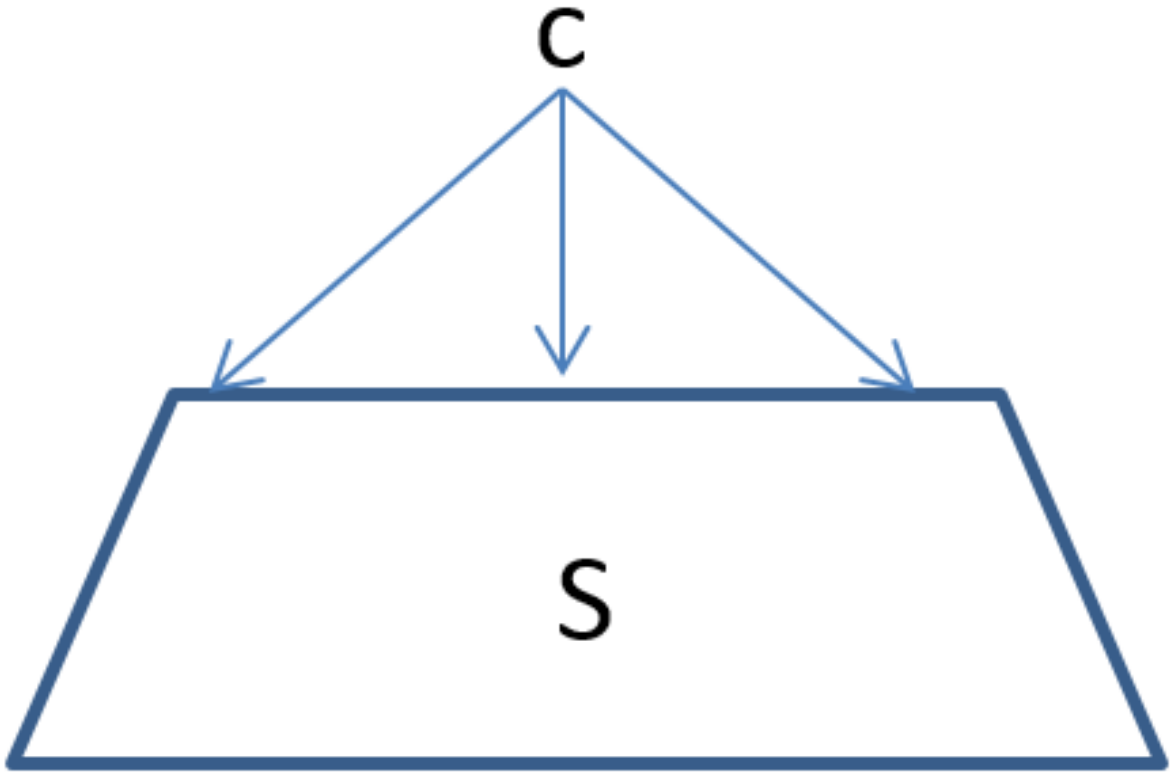
\includegraphics[width=.3\textwidth]{../img/endgame-solving-gadget.png}
  \caption{A~gadget game for endgame solving}
  \label{fig:endgame-solving-gadget}
\end{figure}

\section{Equivalent Linear Program}
The equivalent \acrshort{lp} formulation for the abstracted endgame
\begin{equation*}
  \label{lp:endgame-solving}
  \begin{split}
    \max_{v, x}\  f^\top v & \\
    Ex &= e \\
    F^\top v - A^\top x &\le \vect{0} \\
    x &\ge \vect{0},
  \end{split}
\end{equation*}
is the sequence-form \acrshort{lp} for the gadget game.
Same as in~the \acrshort{lp} from~(\ref{lp:seq-form}):
\begin{itemize}
  \item $A$ is the sequence-form payoff matrix
  \item $x$ is a~vector of~$1$'s sequence probabilities
  \item $v$ is a~vector of~$2$'s (negative) \acrlong{cbv}s
  \item $E$ and $F$ are the sequence constraint matrices 
  \item $e$ is the sequence constraint vector.
\end{itemize}

\section{Discussion}
The endgame solving improves agents' play only \emph{empirically}~(\cite[Table~1]{Ganzfried2015endgame}).
Theoretically, however, there is no guarantee of~optimality:
even if the trunk strategy (and thus the starting distribution) is optimal, the combined strategy can become drastically more exploitable.
This undesired effect is noticeable in~the extensive form of~\acrshort{rps} (Claim~\ref{claim:rps-subgame}, Chapter~\ref{ch:imperf-shortcomings}).

A~worse exploitability arises when the opponent can ``see a~better option'' and aim for it.
This notion of~a~better alternative can be summarized by~a~\emph{counterfactual value}, and Chapter~\ref{ch:cfr-d} shows how to use these values to~guarantee theoretical bounds.

\chapter{CFR-D and Decomposition}
\label{ch:cfr-d}
\note{
  This chapter summarizes the approach, methods and results of~the authors~\cite{BurchJohansonBowling13}.
}

\section{Motivation}
The work of~(\cite{BurchJohansonBowling13}) describes a~pioneering technique how to \emph{decompose} subgames of~imperfect-information games and solve them independently, while preserving the optimality of~the full-game solution.
Many benefits of~subgame re-solving are inherited from perfect-information games:
\begin{itemize}
  \item Run-time information (e.g. endgame actually reached during a~real play) can be exploited in a~smarter way.
  \item Memory and disk limitations (either at~run-time or while solving a~game) can be overcome by a~time/space trade-off.
  \item A~\acrlong{ne} for a~game larger than available storage may be computed.
  \item If we only need to work with one subgame at a~time, then significantly less storage is required.
  \item It is not obligatory to store the complete strategy, which might be too large to store.
    Instead, subgame strategies may be re-computed on~demand, when needed.
\end{itemize}

As for re-solving subgames in~the imperfect-information setting, all previous algorithms were limited to rather small domains, with the complete strategy that can fit in~available space.
As a~consequence, several appealing games still resist to be solved, despite the intensive effort put in~their research.
\note{
  This used to be the case for the two-player \acrshort{lhe}, until the~recent, highly-celebrated breakthrough by~the same research group (\cite{Bowling2015heads}).
}

\section{Gadget Game}
\epigraphLong{
  Dreams about the future are always filled with gadgets.
}{Neil deGrasse Tyson}
Again, we start by~creating a~fine-grained abstraction for the subgame.
The original strategy for the subgame (from the coarse abstraction) is then translated into the fine-grained abstraction as $\sigma_1^S$.
The translated strategy is now used to compute $CBV_2 ^{\sigma_1^S} (I)$ for every information set~$I$ at~the root of~the subgame.
These values will be useful for the gadget construction to~guarantee the safety of~the resulting strategy.
See Figure~\ref{fig:re-solving-gadget} for a~sketch of~the construction.

\begin{figure}[H]
  \centering
  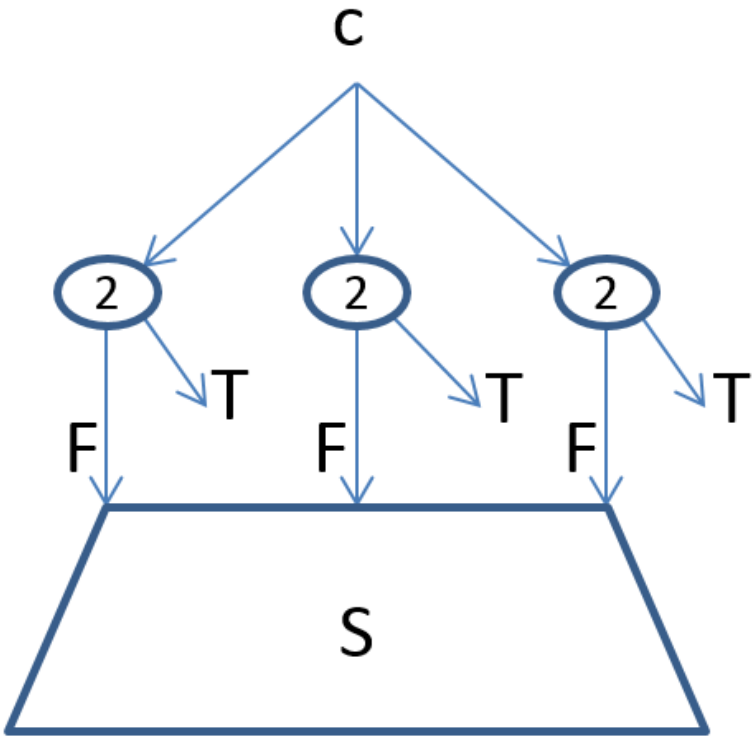
\includegraphics[width=.3\textwidth]{../img/re-solving-game-gadget.png}
  \def\captionTitle{A~gadget game for re-solving subgames}
  \caption[\captionTitle]{
    \captionTitle.
    The opponent chooses in~every state prior to the endgame either to (F)ollow the action into the endgame, or to (T)erminate.
    His utility after the (T)erminal action is set to his counterfactual best response in that state.
  }
  \label{fig:re-solving-gadget}
\end{figure}

To construct the gadget, we add one chance node at~the root of~the game, followed by additional nodes for player~$2$:
one for every state at~the root of the subgame.
At~each of~these nodes, $2$ may either accept the corresponding counterfactual best response value calculated earlier, or play the subgame (to get to the corresponding state at~the root of~the subgame).
The chance player distributes the player~$2$ into these states using the (normalized) $\pi^\sigma_{-2}$ (how likely is the state given that $2$ plays to reach it).
Since the game is zero-sum, this forces player~$1$ to play the subgame well enough, so that the opponent's value is no greater than the original CBV.
For more details see (\cite{BurchJohansonBowling13}).

\section{Equivalent Linear Program}
This time, the presented \acrshort{lp} is not a~straightforward sequential-form representation of~the gadget construction.
Although such a~representation would be possible, it would not help to provide a~desirable insight.
Instead, we formulate an~\acrshort{lp} that solves the same game (for player~$1$) while demonstrating the underlying properties of~the re-solving approach.

The formulation uses the following fact:
any strategy, where the opponent's \acrshort{cbv} is not greater than the original one, is a~solution to the game.
This follows from the construction of~the gadget for re-solving games.

\begin{equation}
  \label{lp:cfr-d}
  \begin{split}
    \max_{v, x}\ &0 \\
    \color{red}
      v_I - m &
    \color{red}
      \ge CBV_2^\sigma(I), \quad I \in \I_2^{R(S)}\\ 
    Ex &= e \\
    F^\top v - A^\top x &\le \vect{0} \\
    x &\ge \vect{0},
  \end{split}
\end{equation}
where $\I_2^{R(S)}$ denotes the root information sets and $CBV_2^\sigma(I)$ is $2$'s original \acrlong{cbv} in~the information set~$I$.
The sequence payoff matrices $A_1$ and $A_2$ are slightly different, to reflect different strategies of~the chance player in the gadget for endgame solving (Figure~\ref{fig:endgame-solving-gadget}) and the gadget for re-solving subgames (Figure~\ref{fig:re-solving-gadget}).

\section{Discussion}
The innovative aspect of~(\cite{BurchJohansonBowling13}) consists of~two main contributions:
\begin{itemize}[(i)]
  \item A~technique to re-solve imperfect-information subgames, which is guaranteed not to increase sub-optimality of~the resulting full-game strategy.
    Owing to summary information about a~subgame strategy (namely the \acrlong{cbv}s), the newly generated strategy is no more exploitable than the original one.

  \item A~new off-line solving algorithm called \emph{\acrfull{cfr-d}}, capable of~computing an~error-bounded \acrshort{ne} approximation.
    \acrshort{cfr-d} achieves this by decomposing and independently analyzing subgames.

    By~sacrificing computation time, the decomposition allows for \emph{sub-linear space costs}.
    For instance, two-player \acrshort{lhe} with \acrshort{cfr-d} can be solved in less than 16 GB, rather than~more than 200 TB of~disk space!
\end{itemize}

\chapter{Subgame-Margin Maximization}
\label{ch:max-margin}
\epigraphLong{
  I have discovered a~truly marvellous proof of~this, which this margin is too narrow to contain.
}{Pierre de Fermat on \emph{Fermat's Last Theorem}}
\vskip -2em
\note{
  This chapter summarizes our own paper~(\cite{Moravcik2016refining}).
}

\section{Motivation and Overview}
The outline of~this chapter is:
\begin{enumerate}[(1)]
    \setlength\itemsep{-.5ex}
  \item listing the steps used by~our technique,
  \item using the problem of~refining imperfect-information subgames to motivate a~value to be maximized,
  \item formalizing this value as the \emph{\acrlong{sm}},
  \item discuss and formalize its properties,
  \item formulate an~\acrshort{lp} optimizing the \acrshort{sm},
  \item describe a~corresponding \acrshort{efg} construction: \emph{a~max-margin gadget}.
\end{enumerate}
Our technique follows the steps of~the subgame-refinement framework:
\begin{enumerate}[(i)]
    \setlength\itemsep{-.5ex}
  \item create an~abstraction for the game;
  \item compute an~equilibrium approximation within the abstraction,
  \item play according to this strategy,
  \item when the play reaches final stage of~the game, create a~fine-grained abstraction for the endgame,
  \item refine the strategy in~the fine-grained abstraction,
  \item use the resulting strategy in that subgame (creating a~combined strategy).
\end{enumerate}
Since all the steps except for (v) are identical to already described techniques, we describe only step (v) in details.

\section{Subgame Margin}
\epigraph{
  Your margin is my opportunity.
}{Jeff Bezos}
To address the potential increase in~exploitability caused by an~opponent altering his behavior in the trunk, we ensure that there is no~distribution of~starting states that would allow him to increase his CBV when confronted by subgame refinement.
The simplest way to ensure this is to decrease his CBV in~all possible starting states.
We can put a~lower bound on~this improvement by measuring the state with the smallest decrease in CBV.
Our goal is to maximize this lower bound.
We refer to this values as the \acrfull{sm}.

\begin{defn}[\acrlong{sm}]
  Let $\sigma_1$, $\sigma_1'$ be a~pair of~player~$1$'s strategies for subgame~$S$.
  Then a~\acrlong{sm}
  \[
    SM_1 (\sigma_1, \sigma_1' , S) =
    \min_{I_2 \in \I_2^{R(S)}}
    \left( CBV_2^{\sigma_1} (I_2) - CBV_2^{\sigma_1'} (I_2) \right)
  \]
  measures the ``gap in~decrease'' between the old and the new \acrlong{cbv}s, across all root information sets $I_2 \in \I_2^{R(S)}$.
\end{defn}

Subgame margin has several useful properties.
The exploitability is strongly related to the value of~the margin:
if it is non-negative, the new combined strategy is guaranteed to be no more exploitable than the original one.
To prove it, we will first re-state Theorem~\ref{thm:cf-val-and-utility} using the following lemma:
\begin{lem}
  \label{lem:cbv-and-sm}
  $CBV_2^{\sigma_1'} (I_2) \leq CBV_2^{\sigma_1} (I_2)$ for all $I_2 \in \I_2^{R(S)}$
  iff
  $SM_1 (\sigma_1, \sigma_1' , S) \geq 0.$
\end{lem}
\begin{proof}
  $
  CBV_2^{\sigma_1'} (I_2) \leq CBV_2^{\sigma_1} (I_2)
  \quad \Longleftrightarrow \quad
  0 \leq CBV_2^{\sigma_1} (I_2) - CBV_2^{\sigma_1'} (I_2)
  \quad \Longleftrightarrow \quad
  0 \leq \min_{I_2 \in \I_2^{R(S)}} \left( CBV_2^{\sigma_1} (I_2) - CBV_2^{\sigma_1'} (I_2) \right)
  = SM_1 (\sigma_1, \sigma_1' , S)
  $
\end{proof}

\begin{cor}[Theorem~\ref{thm:cf-val-and-utility} via \acrlong{sm}]
  \label{cor:sm-and-utility}
  Given a~strategy~$\sigma_1$, a~subgame~$S$, and a~re-solved subgame strategy~$\sigma_1^S$, let $\sigma_1' = \sigma_{1, [S \leftarrow \sigma_1^S]}$ be the combination of~$\sigma_1$ and~$\sigma_1^S$.
  If $SM_1 (\sigma_1, \sigma_1' , S) \geq 0$, then $u_2(\sigma_1', \textrm{CBR}(\sigma_1')) \leq  u_2(\sigma_1, \textrm{CBR}(\sigma_1))$.
\end{cor}

Moreover, given that the opponent's best response reaches the subgame with non-zero probability, the exploitability of~our combined strategy is even reduced.
This improvement is at~least proportional to the subgame margin:

\begin{thm}[improvement proportional to the \acrlong{sm}]
  \label{thm:improvement-propto-sm}
  With the $S$, $\sigma_1$ and $\sigma_1'$ from the Corollary, also assume there exists a~\acrlong{br}~$\sigma_2^* = BR(\sigma_1')$ such that $\pi^{<\sigma_1',\sigma_2^*>} (I_2) > 0$ for some $I_2 \in\I_2^{R(S)}$.
  Then 
  \[
    u_1(\sigma_1', CBR(\sigma_1')) - u_1(\sigma_1, CBR(\sigma_1)) \ge \pi_{-2}^{\sigma_1'} (I_2) \cdot SM_1(\sigma_1, \sigma_1', S).
  \]
\end{thm}
\begin{proof}
  \todo
\end{proof}
Though this lower bound might seem artificial at~first, it has promising properties for the subgame refinement.
Since we refine the strategy once we reach the subgame, either we face $2$'s \acrlong{br} that reaches $S$, or he has made a~mistake earlier in the game.

Furthermore, the probability of~player~$1$ reaching a~subgame is proportional to $\pi_{-2}^{\sigma_1'}(I_2)$.
As this term (and by extension, the bound) grows, the probability of~reaching that subgame increases.
In conclusion, we are more likely to reach a~subgame with a~larger bound.

\section{Linear Program}
To formulate the subgame-margin maximization as an~\acrshort{lp}, we easily modify (\ref{lp:cfr-d}):
\begin{equation}
  \label{lp:max-margin}
  \begin{split}
    \max_{v, x}\ &\textcolor{red}{m} \\
    v_I - m &\ge CBV_2^\sigma(I), \quad I \in \I_2^{R(S)}\\ 
    Ex &= e \\
    F^\top v - A_2^\top x &\le \vect{0} \\
    x &\ge \vect{0},
  \end{split}
\end{equation}
where $m$ is a~scalar corresponding to the subgame margin that we aim to~maximize.
It serves as ``a gap'' between all values $v_I$ and the given constants $CBV_2^\sigma(I)$, and we wish to make this gap as~large as~possible.

The similarities between (\ref{lp:max-margin}) and (\ref{lp:cfr-d}) make it easier to see our improvement:
whereas the \acrshort{lp} (\ref{lp:cfr-d}) only guarantees a~non-negative margin, we maximize it.
Although the optimization formulation is almost identical to~the re-solving, our gadget construction is different.

\section{Equivalent Gadget Game}
\epigraphLong{
  A~new gadget that lasts only five minutes is worth more than an~immortal work that bores everyone.
}{Francis Picabia}
One way to find the refined strategy is to solve the corresponding \acrfull{lp}.
However, algorithms that are tailor-made for \acrshort{efg}s often outperform the optimization approach (\cite{Bosansky2013solving}).
These algorithms often permit the use of~domain-specific tricks to provide further performance gains (\cite{Johanson2012efficient}).
Thus, formulating our optimization problem~(\ref{lp:max-margin}) as an \acrshort{efg} will mean that we can compute larger subgame abstractions using the available computing resources.
Essentially, the construction of a~gadget game equivalent to the \acrshort{lp}~(\ref{lp:max-margin}) will allow us to compute larger subgames---more than it would be possible with just the plain \acrshort{lp}.

All states in~the original subgame are directly copied into the resulting gadget game.
We create the gadget game by~making two alterations to~the original subgame:
\begin{enumerate}[(i)]
  \item we shift player~$2$'s utilities using the $CBV_2$ (to initialize all $2$'s values to~zero)
  \item we add a~rooting node~$\dt$ for $2$, followed by chance nodes $c_{I_1}, c_{I_2}, c_{I_3}, \dots$ at~the top of the subgame (to allow the opponent to~pick any starting state, relating the game values to~the margin)
\end{enumerate}

\begin{figure}[H]
  \centering
  \def\svgwidth{.4\textwidth}
  \input{../img/max-margin-gadget.pdf_tex}
  \def\captionTitle{Our max-margin gadget}
  \caption[\captionTitle]{\captionTitle. When $1$'s original strategy is used, the terminal nodes' offsets enforce the opponent to have a~zero utility in~best response.}
  \label{fig:max-margin-gadget}
\end{figure}

The following is a~description of~the steps (see also Figure~\ref{fig:max-margin-gadget} that visualizes the gadget).
\begin{enumerate}
  \item We establish a~common baseline.
    For~comparing changes in~the performance of~$2$'s root information sets, they need a~common starting point:
    the original strategy $\sigma_1^S$.

    For every $I \in \I_2^{R(S)}$ we subtract the opponent's original \acrlong{cbv}, setting the utility at~each terminal node~$z \in Z(I)$ to $\ut_2(\zt) = u_2(z) - CBV_2^{\sigma^S_1}(I)$.
    We must not forget to~update $\ut_1(\zt) = -\ut_2(\zt)$ either, as we need the game to remain zero-sum.
    Conditioned on~the original strategy $\sigma_1^S$, the shifting gives an~expected value of~$0$ to~opponent's starting states.

  \item Player~$2$ is permitted to choose his belief at~the start of~the subgame, while $1$ retains his belief from the original strategy at~the starting point of~the subgame.
    Since $2$ is aiming to~maximize $\ut_2$, he will always select the information set with the lowest margin.
    The minimax nature of~the zero-sum game motivates player~$1$ to find a~strategy maximizing this value of~the lowest margin.

    We create an~additional decision node $\dt$ for player~$2$.
    Every action corresponds to choosing an~initial information set $I\in \I_2^{R(S)}$.
    However, since an~action can lead only to a~single tree node rather than a~whole information set, we may not connect this action to state~$\dt$ directly.
    Instead, each action leads to a new chance node $c_{\It}$, where the chance distributes histories~$\htil \in \It$ based on~the probability~$\pi_{-2}^\sigma (h)$.

    \todo
\end{enumerate}

Following from the construction, we get straightforwardly
\begin{claim}
  A~strategy for the max-margin gadget is a~\acrlong{ne} if and only if it is a~solution to the \acrshort{lp}~(\ref{lp:max-margin}).
\end{claim}

\section{Gadget Game Revisited}
First of~all, we show that re-solving does not increase \acrshort{cbv}s at~the root of the subgame, when compared to old \acrshort{cbv}s in the original game.

Let $\mathcal{I}_2^{R(S)}$ be the set of~information sets at~the root of a~subgame~$S$ and let $\sigma$ be the strategy from the original game.
On top of that, for every information set~$I~\in~\mathcal{I}_2^{R(S)}$ we are given its \acrlong{cbv} $CBV_2^{\sigma}(I)$.

We construct a~new two-player zero-sum perfect-recall ``gadget'' game $\tilde{S}$.
First, we add a~new root node $\dt$, where the opponent chooses an~information set $I \in \mathcal{I}_2^{R(S)}$ to enter.
\hrule
\todo
Formally, this can be achieved by creating chance nodes $\tilde{r}_I$ per each set $I \in \mathcal{I}_2^{R(S)}$.
As soon as the opponent chooses which $\tilde{r}_I$ to enter, the chance player deals our cards.
Namely, for each $\tilde{h}\in I$, the chance to be in state $h$ is determined as
$\pi_c (\tilde{r}_I, \tilde{r}_I \cdot \tilde{h}) = \pi_{-2} ^{\sigma}(\tilde{h}) / k_I$.
Here, the normalization factor $k_I = \sum_{ \tilde{h} \in I} \pi_{-2}^\sigma(\tilde{h})$ is used in order to make probabilities
$\pi_c (\tilde{r}_I, \tilde{r}_I \cdot \tilde{h})$ sum to $1$ within any information set $I \in I_2 ^{R(S)}$.

The remaining structure of the subgame is directly copied, replicating every state $h$ with a~state $\tilde{h}$.
On top of that, the utility of every terminal node is shifted by the counterfactual value of the containing root information set.
That is, for all $I \in \mathcal{I}_2^{R(S)}$ and all terminal $z \in Z(I)$, the utility is set to
$\tilde{u}_2(z) := k_I \cdot \left(u_2(z) - v_2(I)\right)$ if we also take into account the normalization factor.
Thus, we get
\begin{lem}
  \label{lem:cfshift}
  For each $I\in\mathcal{I}_2^{R(S)}$, the corresponding counterfactual value is
  $\tilde{v}_2 ^\tilsig(I) = v_2 ^{\sigma'}(I) - v_2(I)$
  under any subgame strategy profile $\tilsig$ and its extension
  $\sigma' = \sigma_{[S \leftarrow \tilsig]}$ to the original game.
\end{lem}

\begin{proof}
  The counterfactual value in the gadget game is
  \begin{equation*}
    \begin{split}
      \tilde{v}_2^\tilsig (I)
      &= \sum_{z\in Z(I)}
      \pi_{-2}^\tilsig(\dt, z) 
      \cdot \pi_{2}^\tilsig(z[I], z)
      \cdot \tilde{u}_2(z) \\
      &= \sum_{z\in Z(I)}
      \frac{\pi_{-2}^{\sigma}(z[I])}{k_I}
      \cdot \pi^{\tilde{\sigma}}(z[I], z)
      \cdot \tilde{u}_2(z) \\
      &= \sum_{z\in Z(I)}
      \pi_{-2}^{\sigma'}(z[I])
      \cdot \pi^{\sigma'}(z[I], z)
      \cdot (u_2(z) - v_2(I)) \\
      &= v_2^{\sigma'}(I) - \sum_{z\in Z(I)}
      \pi_{-2}^{\sigma'}(z) 
      \cdot \pi_{2}^{\sigma'}(z[I], z)
      \cdot v_2(I) \\
      &= v_2 ^{\sigma'}(I) - v_2(I).
    \end{split}
  \end{equation*}
  The last equality holds because behavior strategies $\sigma'$ define some probability distribution in each tree node.
  Therefore by induction, we get $\sum_{z\in Z(I)} \pi_{-2}^{\sigma'}(z) \cdot \pi_{2}^{\sigma'}(z[I], z) = 1$.
\end{proof}

Now we prove that our gadget game does not increase the counterfactual values in the root information sets:
\begin{thm}
  \label{thm:cf-val-max-margin-gadget}
  Let us have the original strategy $\sigma_1$ of player~$1$, a~subgame~$S$, and a~re-solved subgame strategy $\sigma_1^S$ for the above-constructed gadget game.
  Let also $\sigma_1' = \sigma_{1, [S \leftarrow \sigma_1^S]}$ be the combination of $\sigma_1$ in the trunk and $\sigma_1^S$ in the subgame~$S$.
  Then $v_2^{\langle\sigma_1', \textrm{CBR}(\sigma_1')\rangle}(I) \leq  v_2^{\langle\sigma_1, \textrm{CBR}(\sigma_1)\rangle}(I) \equiv v_2(I)$ holds for every information set $I\in\mathcal{I}_2^{R(S)}$ at the root of subgame $S$.
\end{thm}

\begin{proof}
  Note that player $1$ could decide to play the original $\sigma'_1 := \sigma_1$ in the constructed game.
  Together with the opponent's best response $\textrm{CBR}_2(\sigma'_1) = \textrm{CBR}_2(\sigma_1)$, we obtain the strategy profile 
  $\sigma' := \langle \sigma_1, \textrm{CBR}_2(\sigma_1) \rangle$.
  It yields the identical counterfactual values
  $v_2 ^{\sigma'} (I) = v_2(I)$ for all $I\in\mathcal{I}_2^{R(S)}$.
  By Lemma \ref{lem:cfshift}, with $\tilsig'$ as the subgame portion of~the whole $\sigma'$, the counterfactual values evaluates to
  $\tilde{v}_2 ^{\tilsig'}(I)
  = v_2 ^{\sigma'} (I)~-~v_2(I)
  = v_2(I)~-~v_2(I)
  =~0$.

  Since any counterfactual value of a~root is the same thing as the regular expected value, we infer that
  \begin{equation*}
    \begin{split}
      \tilde{u}_2 ^{\tilsig'} (\dt)
      &= \tilde{v}_2 ^{\tilsig'} (\dt)
      = \max _{I\in \mathcal{I}_2^{R(S)}} \tilde{v}_2 ^\tilsig (\tilde{r}_I) \\
      &= \max _{I\in \mathcal{I}_2^{R(S)}} \tilde{v}_2 ^\tilsig (I)
      = \max _{I\in \mathcal{I}_2^{R(S)}} 0 
      = 0,
    \end{split}
  \end{equation*}
  where the second equality is due to the best-response property.
  In a~zero-sum game, this means 
  $
  \tilde{u}_1 ^{\tilsig'} (\dt)
  = - \tilde{u}_2 ^{\tilsig'} (\dt)
  = 0
  $,
  and thus, the maximizing player~$1$ can only do better.
  In particular, he gains utility
  $
  \tilde{u}_1 ^{\sigma^S} (\dt) \ge 0
  $
  for some optimal strategy $\sigma_1^S$ and the corresponding profile
  $\sigma^S := \langle \sigma_1^S, \textrm{CBR}_2 (\sigma_1^S)\rangle$,
  which implies
  \begin{equation*}
    \begin{split}
      0
      &\ge - \tilde{u}_1 ^{\sigma^S} (\dt)
      = \tilde{u}_2 ^{\sigma^S} (\dt)
      = \tilde{v}_2 ^{\sigma^S} (\dt) \\
      &= v_2 ^{\langle\sigma_1', \textrm{CBR}(\sigma_1')\rangle} (I)~-~v_2(I)
    \end{split}
  \end{equation*}
  using again Lemma \ref{lem:cfshift} for the last equality.
  Finally, the inequality translates to the desired
  $
  v_2 ^{\langle\sigma_1', \textrm{CBR}(\sigma_1')\rangle} (I) \le v_2(I).
  $
\end{proof}

\begin{cor}
  \label{cor:sm-max-margin-gadget}
  \todo
\end{cor}

\todo
Moreover, not only the counterfactual values cannot get increased, but the construction also ensures that the gap between the old and new ones is as large as possible.
On top of that, not only the construction preserves the upper bounds of~counterfactual values, it maximizes the gap between them and their previous values:

\begin{thm}
  \label{thm:sm-maximized}
  In the same setting as in Theorem \ref{thm:nyx-cfval}, the margin
  \[
    m := \min _{I \in \mathcal{I}_2^{R(S)}} 
    \left( v_2(I) - v_2^{\langle\sigma_1', \textrm{CBR}_2 (\sigma_1')\rangle}(I) \right)
  \]
  is maximum among all possible $\sigma'_1$.
\end{thm}
\begin{proof}
  For a~contradiction, let there be a~strategy profile~$\ovsigma = \langle \ovsigma_1, \textrm{CBR}_2 (\ovsigma_1)\rangle$, which is the strategy $\sigma$ with substituted subgame part and which generates a~better margin
  \[
    m' := \min _{I \in \mathcal{I}_2^{R(S)}} 
    \left( v_2(I) - v_2^{\ovsigma}(I) \right)
    > m.
  \]
  To get a~counterfactual best response $\textrm{CBR}_2 (\ovsigma_1)$, player~$2$ may only mix the actions with the largest counterfactual values.
  In state $\dt$ this means
  \begin{equation*}
    \begin{split}
      \tilde{u}_2 ^\ovsigma(\dt)
      &= \tilde{v}_2 ^\ovsigma(\dt)
      = \max _{I \in \mathcal{I}_2^{R(S)}} \tilde{v}_2 ^\ovsigma(I)
      = - \min _{I \in \mathcal{I}_2^{R(S)}} \left( -\tilde{v}_2 ^\ovsigma(I) \right) \\
      &= - \min _{I \in \mathcal{I}_2^{R(S)}} \left( v_2(I) - v_2^{\ovsigma}(I) \right)
      = - m'
    \end{split}
  \end{equation*}
  where the penultimate equality is justified by Lemma~\ref{lem:cfshift}.

  In a~zero-sum game, we get
  $
  \tilde{u}_1 ^\ovsigma(\dt)
  = -\tilde{u}_2 ^\ovsigma(\dt)
  = m'
  $,
  Similarly,
  $
  \tilde{u}_1 ^{\langle\sigma_1', \textrm{CBR}(\sigma_1')\rangle} (\dt)
  = m
  $
  by an~analogous transcription.
  In conclusion, this implies
  $
  \tilde{u}_1 ^\ovsigma(\dt)
  > \tilde{u}_1 ^{\langle\sigma_1', \textrm{CBR}(\sigma_1')\rangle} (\dt)
  $,
  which contradicts the fact that $\langle\sigma_1', \textrm{CBR}(\sigma_1')\rangle$ is a~Nash equilibrium in the gadget game~$\tilde{S}$.
\end{proof}

The previous theorem suggests that our construction has a~counterpart in~the form of~a sequence-form linear program.
Indeed, it is intuitively equivalent to the LP~(\ref{lp-nyx}), as the solution to the gadget game maximizes the margin in counterfactual values.
This is an~improvement over the approach demonstrated by~(\cite{BurchJohansonBowling2014}).

\section{Experimental Results}
\label{sec:max-margin-experiments}
\epigraphLong{
  If you find that you're spending almost all your time on theory, start turning some attention to practical things; it will improve your theories. If you find that you're spending almost all your time on practice, start turning some attention to theoretical things; it will improve your practice.
}{Donald Knuth}
In this section, we evaluate endgame solving (Chapter~\ref{ch:endgame-solving}), subgame re-solving (Chapter~\ref{ch:cfr-d}) and max-margin subgame refinement (this chapter) on~the safe-refinement task for a~large-scale game.
We use an~improved version of~the \emph{Nyx} agent, the second strongest participant at~the 2014 \emph{Annual Computer Poker Competition} (\acrlong{nlhe} Total Bankroll)\footnotemark{} as~the baseline strategy to be re-fined in~subgames.
\footnotetext{\href{http://www.computerpokercompetition.org/index.php/competitions/results/105-2014-results}{http://www.computerpokercompetition.org/index.php/competitions/results/105-2014-results}}

All three of~the subgame refinement techniques tested here used the same abstractions and trunk strategy.
Following (\cite{Ganzfried2015endgame}), we begin the subgame at~start of~the last round (the river).
Although we used card abstraction to compute the original trunk strategy (\cite{Schmid2015automatic, Johanson2013evaluating}), the fine-grained abstraction for the endgame is calculated \emph{without the need for card abstraction}.
This is an~improvement over the original implementation of~(\cite{Ganzfried2015endgame}), where both the trunk strategy and the refined subgame used card abstraction.
This is a~result of~the improved efficiency of~the \cfrplus algorithm (and the domain-specific speedups it enables), whereas the endgame solving of~(\cite{Ganzfried2015endgame}) used linear programming to~compute the strategy.

The original strategy uses action abstraction with up to $16$ actions in~an~information set.
While this number is relatively large compared to other participating agents, it is still well below the best-known upper bound on~the optimal strategy's  support size (\cite{Schmid2014bounding}).
The action abstraction used for the original Nyx strategy has the imperfect recall, whereas the refined subgame uses the perfect recall.
We use the same actions in~the refined subgame as in~the original strategy.

We refine only the subgames that has less than $1000$ betting sequences (after creating the fine-grained abstraction).
This is simply to speed up the experiments.
The original agent's strategy is preserved in~the trunk of~the game for both player~$1$ and player~$2$.
Once gameplay reaches the subgame (the river), we refine $1$'s strategy using each of~the three techniques.
We have run $10000$ iterations of~the \cfrplus algorithm in the corresponding gadget games, with exponential weighting to update the average strategies (\cite{Tammelin2015solving}).
Each technique was used to refine $\approx 2000$ subgames.
Figure~\ref{fig:sm-experiments} displays the average margins for the evaluated techniques.

The max-margin technique produces the optimal value, much greater than ones produced by~subgame re-solving or endgame solving (which has even negative \acrlong{sm}s).

\begin{figure}[H]
  \centering
  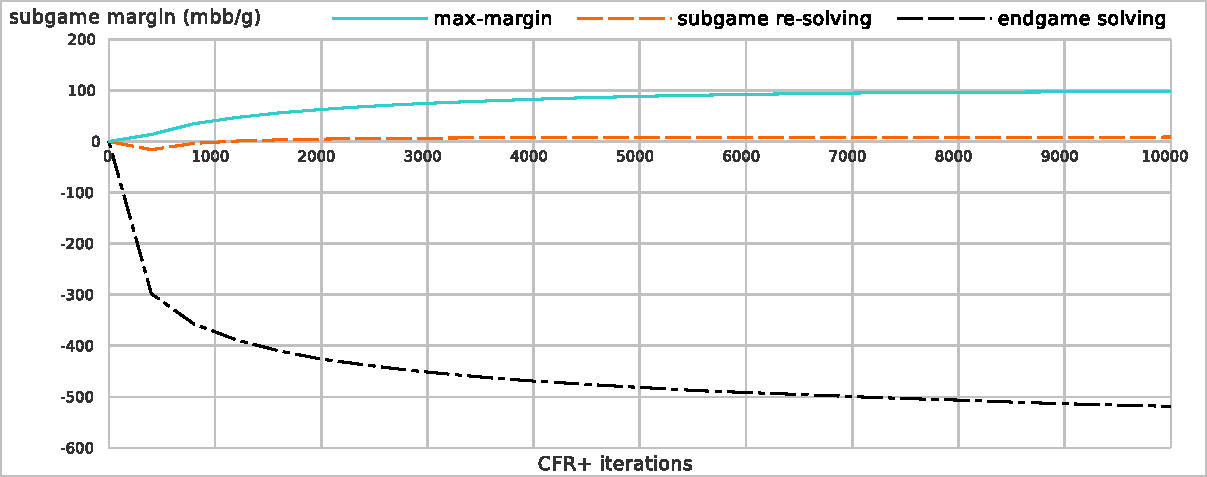
\includegraphics[width=\textwidth]{../img/sm-experiments}
  \def\captionTitle{\cfrplus iterations versus \acrshort{sm} of~refined strategies}
  \caption[\captionTitle]{\captionTitle (in milli big blinds per game).
    One big blind corresponds to 100 chips.
  }
  \label{fig:sm-experiments}
\end{figure}

The $95\%$ confidence intervals after $10000$ iterations are
\begin{itemize}
  \item max-margin: $101.49 \pm 7.09$
  \item subgame re-solving: $8.79 \pm 2.45$
  \item endgame solving: $-518.5 \pm 49.19$
\end{itemize}

\chapter{Ideas for Future Work}
\label{ch:future-work}
\epigraphLong{
  The worst thing that can happen in a~democracy---as well as in an~individual's life---is to become cynical about the future and lose hope.
}{Hillary Clinton}
One may try to study other aspects of~endgames.
Some recommendations as inspiration for future work may include
\begin{itemize}
  \item other endgame-specific concepts like \acrlong{sm}
  \item dynamical adjustment of~computation upon entering the ending phase
  \item solving several endgames in~parallel, without interdependence
  \item a~Poker version of~Chess endgame tablebases, which poker agents may use in~simpler ending situations to play perfectly
\end{itemize}

\section{Margins via Multi-Objective Optimization}
\epigraphLong{
  Raise your quality standards as~high as you can live with, avoid wasting your time on~routine problems, and always try to~work as~closely as~possible at~the boundary of~your abilities.
  Do this, because it is the only way of~discovering how that boundary should be moved forward.
}{Edsger Dijkstra}
One especially noteworthy research topic is the study of~margins (i.e., declines of~\acrshort{cbv}s).
The \acrlong{sm} is their $\min$-aggregation.
Tempting idea is to look into alternative aggregations.
Consider a~multi-criteria analogy to~subgame margin maximization (\ref{lp:max-margin}):
\begin{equation}
  \label{vlp:max-margins}
  \begin{split}
    \max_{v, x}\ &\textcolor{red}{\vect{m}} \\
    v_I - \vect{m}_{\textcolor{red}{I}} &\ge CBV_2^{\sigma_1}(I), \quad I \in \I_2^{R(S)}\\ 
    Ex &= e \\
    F^\top v - A_2^\top x &\le \vect{0} \\
    x &\ge \vect{0}.
  \end{split}
\end{equation}
Now $\vect{m}_I$ corresponds to one specific margin $\vect{m}_I := CBV_2^{\sigma_1} (I) - CBV_2^{\sigma_1'} (I)$, and $\vect{m} := (m_I) _{I\in\I_2^{R(S)}}$ is a~vector of~all such margins.
Evidently, this \acrfull{vlp} is a~task of~\emph{multi-objective optimization} (\cite{Ehrgott2006multicriteria, Grygarova1996zaklady}).

Notice that (\ref{lp:max-margin}) is just a~special case of~the vector objective function, by~the scalarization
\[
  \max_{v, x}\ \min_{I \in \I_2^{R(S)}}\ {\vect{m}_I}.
\]
The choice of~minimum function stems from the nature of~the opponent, who makes his best to exploit us and hence aims for minimal decrease in~\acrshort{cbv}s.

Undoubtedly, one can also try other methods to deal with multi-objective functions:
\begin{itemize}
  \item other scalarizations, e.g., weighted sum of~margins
  \item (Pareto) efficient solutions
  \item \acrfull{dea}:
    \href{http://www.deazone.com/}{http://www.deazone.com/}
  \item \acrfull{emo}, which uses evolutionary algorithms:
    \href{https://www.cs.cinvestav.mx/~EVOCINV/}{https://www.cs.cinvestav.mx/$\sim$EVOCINV/}
\end{itemize}
It might be compelling as well as intriguing to understand their meaning in~the language of~\acrlong{efg}s, and perhaps even find their corresponding gadget games.

%%%%%%%%%%%%%%%

\chapter*{Conclusion}
\addcontentsline{toc}{chapter}{Conclusion}
\epigraphLong{
  Everything that civilisation has to~offer is a~product of human intelligence;
  we cannot predict what we might achieve when this intelligence is magnified by~the tools that AI may provide, but the eradication of~war, disease, and poverty would be high on~anyone's list.
  Success in~creating AI would be the biggest event in~human history.
  Unfortunately, it might also be the last.
}{Stephen Hawking}
Perfect-information endgames can be solved by backward induction, where solutions to subgames are propagated up the game tree.
For the imperfect information, on~the other hand, endgames need to be adjusted in~order to account for information sets.
This gives rise to a~new definition of~an~(imperfect-information) \emph{subgame}.
As such, the definition does not directly allow to apply the same procedure as in~perfect-information endgames:
under even the simplest conditions of~the \acrlong{rps} game, a~na{\"i}ve endgame re-solution fails to form a~\acrlong{ne}.

This occurs because the opponent can change his behavior prior to the endgame.
Such an~exploitation power can be captured by~a~\emph{counterfactual value}:
a~hypothetical ``what-if'' value summarizing opponent's improvement, if he had changed his prior trunk strategy.

We used counterfactual values to define our own notion of~\emph{\acrlong{sm}}:
a~gap between the original and the new \acrlong{cbv}s.
We related the \acrshort{sm} to the exploitability against a~\acrlong{br}, and we proved the overall improvement rising from endgame improvement is proportional to the \acrshort{sm}.

Maximizing \acrshort{sm} is thus highly advisable.
That can be achieved either by solving a~variant of a~sequence-form \acrlong{lp}, or by applying an~iterative learning algorithm to a~\emph{gadget game}, an~equivalent ad-hoc \acrlong{efg}.
The latter approach offers greater benefits in~terms of~exploiting domain-specific knowledge and employing powerful learning algorithms such as \acrshort{cfr}, \acrshort{mccfr} or the~modern \cfrplus{} that we chose to solve our \emph{max-margin gadget}.

Finally, we experimentally compared the three contemporary approaches to solving endgames:
\begin{enumerate}[(i)]
  \item endgame solving (\cite{Ganzfried2015endgame})
  \item \acrshort{cfr-d} and decomposition (\cite{BurchJohansonBowling2014})
  \item our subgame-margin maximization (\cite{Moravcik2016refining})
\end{enumerate}
The results of~the experiments showed that (i) even produced a~worse \acrshort{sm}, leading to more exploitable subgame strategies;
and although the \acrshort{sm} of~(ii) increased over time, the improvement was not significant, as the method guarantees only the same (or comparable) quality, not the best one.
Since our (iii) was specially designed to maximize \acrshort{sm}s, it re-created the most robust (i.e., the least exploitable) subgame strategy.
We thus offer a~superior solution to treating subgames.


%%% Bibliography
%%% Bibliography (literature used as a source)
%%%
%%% We employ bibTeX to construct the bibliography. It processes
%%% citations in the text (e.g., the \cite{...} macro) and looks up
%%% relevant entries in the bibliography.bib file.
%%%
%%% The \bibliographystyle command selects, which style will be used
%%% for references from the text. The argument in curly brackets is
%%% the name of the corresponding style file (*.bst). Both styles
%%% mentioned in this template are included in LaTeX distributions.

\bibliographystyle{plainnat}    %% Author (year)
% \bibliographystyle{unsrt}     %% [number]

\renewcommand{\bibname}{Bibliography}

%%% Generate the bibliography. Beware that if you cited no works,
%%% the empty list will be omitted completely.

\bibliography{bibliography}

%%% If case you prefer to write the bibliography manually (without bibTeX),
%%% you can use the following. Please follow the ISO 690 standard and
%%% citation conventions of your field of research.

% \begin{thebibliography}{99}
%
% \bibitem{lamport94}
%   {\sc Lamport,} Leslie.
%   \emph{\LaTeX: A Document Preparation System}.
%   2nd edition.
%   Massachusetts: Addison Wesley, 1994.
%   ISBN 0-201-52983-1.
%
% \end{thebibliography}


%%% Figures used in the thesis (consider if this is needed)
\listoffigures

%%% Tables used in the thesis (consider if this is needed)
%%% In mathematical theses, it could be better to move the list of tables to the beginning of the thesis.
\listoftables

%%% Abbreviations used in the thesis, if any, including their explanation
%%% In mathematical theses, it could be better to move the list of abbreviations to the beginning of the thesis.
\setglossarystyle{list}
\printglossary[title=List of~Abbreviations, toctitle=List of~Abbreviations, type=\acronymtype]

%%% Attachments to the master thesis, if any. Each attachment must be
%%% referred to at least once from the text of the thesis. Attachments
%%% are numbered.
%%%
%%% The printed version should preferably contain attachments, which can be
%%% read (additional tables and charts, supplementary text, examples of
%%% program output, etc.). The electronic version is more suited for attachments
%%% which will likely be used in an electronic form rather than read (program
%%% source code, data files, interactive charts, etc.). Electronic attachments
%%% should be uploaded to SIS and optionally also included in the thesis on a~CD/DVD.
%\chapwithtoc{Attachments}

%%%% for abstract in Czech
\thispagestyle{empty}
\openright

\vbox to 0.5\vsize{
\setlength\parindent{0mm}
\setlength\parskip{5mm}

Název práce:
{\let\\=\relax \ThesisTitle}

Author:
\ThesisAuthor

\DeptType:
\Department

Supervisor:
\Supervisor, \SupervisorsDepartment

Abstract:
\Abstract

Keywords:
\Keywords

\vss}

\newpage


\openright
\end{document}
